%% Maybe abbreviate PBN.

% Ijcai thoughts:
% say that this works well with ensemble methods.
% rev up the rhetoric
% mention StarAI workshop?
% maybe tone down the acyclicity.
% If you want to use conditional probs, need to scale
% from Greg: strong baseline method

\documentclass[twoside,leqno,twocolumn]{article}
\usepackage{ltexpprt}

%Example for automatically rescaling equations. 
% This is very tricky.
%\begin{equation}
%\label{eq:pimax}
%\resizebox{.55\textwidth}{!}{$
%\begin{split}
%P(\jtable_{2}|\set{E},\ttable) \propto &
%P(\keys = [jack,101],\it{Gr} = A, \it{Sat} = 1|\it{Int} = \class, \it{Rank} = 1, \it{Rat} = 3, \it{Diff}=1)\\
%\times & P(\keys = [jack,102],\it{Gr} = B, \it{Sat} = 2|\it{Int} = \class, \it{Rank} = 1, \it{Rat} = 2, \it{Diff}=2).
%\end{split}$
%}
%\end{equation}

%\usepackage{times}
%\usepackage[normaltitle,normalbib,normalmargins,normalindent]{savetrees}
\usepackage{amsmath}
\usepackage{amsfonts}
\usepackage{amssymb}
\usepackage{graphicx}
\usepackage{url}
%\usepackage{subfigure}
\usepackage{epstopdf}
\setcounter{MaxMatrixCols}{30}
%\usepackage{algorithm}
%\usepackage{algorithmic}
\usepackage{subfigure}
%\usepackage{subcaption}
\usepackage{fancyhdr}
\graphicspath{{../}{figures/}}
\usepackage{todonotes}

\DeclareMathOperator*{\argmax}{argmax}
\DeclareMathOperator*{\argmin}{argmin}
%\DeclareMathOperator{\pattern}{\pi}
\DeclareMathOperator{\Poly}{\mathbf{\mathrm{P}}}
\DeclareMathOperator{\RP}{\mathbf{\mathrm{RP}}}
%\DeclareMathOperator{\FP}{\mathbf{\mathrm{FP}}}
\DeclareMathOperator{\NP}{\mathbf{\mathrm{NP}}}
%\DeclareMathOperator{\E}{\mathbb{E}}
\renewcommand{\d}{\mathbf{d}}

\newcommand{\ZZ}{\mathbf{Z}}

\newcommand{\indep}{\ensuremath{\perp{}\!\!\!\!\!\!\!\perp{}}}
\newcommand{\dep}{\ensuremath{{\perp{}\!\!\!\!\!\!\!\not  \perp{}}}}
%\renewcommand{\L}{\mathcal{L}}
% variables denoting sets of nodes
\newcommand{\V}{V} 
\newcommand{\partC}{\mathcal{C}}
\newcommand{\pattern}{\pi}
% variables denoting nodes
\newcommand{\B}{B}
\renewcommand{\P}{P}
\newcommand{\R}{R}
\newcommand{\X}{X}
\newcommand{\Y}{Y}
\newcommand{\Z}{Z}
\newcommand{\F}{F}
\newcommand{\U}{U}
\newcommand{\W}{W}
\renewcommand{\S}{S}
\newcommand{\C}{C}
\newtheorem{mydef}{Proposition}
%variables for values
%\newcommand{\u}{u}
\renewcommand{\a}{a}
\renewcommand{\b}{b}
\newcommand{\z}{z}
\renewcommand{\v}{v}
\newcommand{\x}{x}
\newcommand{\y}{y}
\newcommand{\p}{p}
\newcommand{\s}{s}
\newcommand{\w}{w} % weights


%statistics
\newcommand{\divergence}{\it{D}}
\newcommand{\score}{\it{score}}
\newcommand{\confidence}{\it{conf}}
\newcommand{\support}{\it{support}}
\newcommand{\loglikelihood}{\it{LOG}}
\newcommand{\lof}{\it{LOF}}
\newcommand{\llmetric}{-L}
\newcommand{\lr}{\it{LR}}
\newcommand{\kl}{\it{KL}}
\newcommand{\el}{\it{EL}}
\newcommand{\mi}{\it{MI}}
\renewcommand{\mid}{\it{ELD}}
\newcommand{\jid}{\it{JID}}
\newcommand{\roc}{\it{ROC}}
\newcommand{\outrank}{\it{OutRank}}
\newcommand{\knn}{\it{KNNOutlier}}
\newcommand{\auc}{\it{AUC}}
\newcommand{\eld}{\it{ELD}}
\newcommand{\fd}{\it{FD}}
\newcommand{\parameter}{\theta}
\newcommand{\parameters}{\bs{\parameter}}
\newcommand{\bic}{\mathit{BIC}}
%random variables and graphical models
% number of values in the domain of a random variable
% variables for BNs
\newcommand{\domvals}{k}
\newcommand{\nodevalue}{\v}
\newcommand{\parvalue}{\mathbf{\pi}} % a single assignment of values to a set of 
%parents
\newcommand{\parvals}{l} % number of values of parent state.
\renewcommand{\r}{r} % CP-table row
\newcommand{\nbhd}{{\mathsf {nbdh}}}
\newcommand{\child}{\mathit{child}}
\newcommand{\parent}{\mathit{pa}}
\newcommand{\parents}{\mathbf{pa}}
\newcommand{\Parents}{\mathbf{PA}}
\newcommand{\family}{F} % families, family formulas
\newcommand{\vpi}{\mathbf{pa}} % for vectors of variable assignments
\renewcommand{\l}{\ell} % class label
\newcommand{\states}{r} % number of states of a variable
%\newcommand{\value}{value}
\newcommand{\mb}{\set{mb}} % markov blanket of a variable, vector-valued
\newcommand{\ssize}{N} % number of rows in join table; size of sample
\newcommand{\mbstates}{m} % number of states in Markov blanket
\newcommand{\frequency}{fr}
\newcommand{\pseudo}{\ast}
\newcommand{\counts}{+}
\newcommand{\weighted}{\ast}
\newcommand{\halpern}{H}
\newcommand{\Thetaa}{\theta}
\newcommand{\instance}{I}

%logic notation
%\newcommand{\predicate}{\phi}
\newcommand{\functor}{f}
\newcommand{\outdomain}{V}
\newcommand{\indomain}{\Omega}
\newcommand{\variable}{X} % first-order variable
\newcommand{\population}{\mathcal{P}}
\newcommand{\entity}{x}
\newcommand{\formula}{\phi}
\newcommand{\formulas}{\mathcal{\phi}}
\newcommand{\literal}{l}
\newcommand{\conjunction}{\set{C}} % conjunction of literals
\newcommand{\fterm}{\f} % open function term
\newcommand{\fterms}{F} % set of function terms, also nodes in JBN
\newcommand{\term}{\sigma}
\newcommand{\Terms}{\bs{\sigma}}
\newcommand{\constant}{a}
\newcommand{\constants}{\bs{\constant}}
\newcommand{\gterm}{g} % ground term
\newcommand{\gterms}{\bs{\gterm}} %list of ground terms
\newcommand{\vterm}{x} % variable term
\newcommand{\vterms}{\bs{\vterm}} % list of variable terms
\newcommand{\assign}{A} % assignment of values to Bayes net
\newcommand{\resultset}{\mathbb{R}}
\newcommand{\grounds}{\#}
\newcommand{\grounding}{\gamma}
\newcommand{\groundall}{\Gamma}
\newcommand{\vars}{\mathit{Var}} % variables in a conjunction
\newcommand{\igraph}{I} % instance-level dependency graph.
\newcommand{\assignment}{\set{a}}
\newcommand{\atom}{\ell}
\newcommand{\gnode}{\alpha}
\newcommand{\gfamily}{\ground{f}}
\newcommand{\numformulas}{m}
\newcommand{\structure}{\mathcal{S}}
% logic programs
\newcommand{\program}{\mathcal{B}}
\newcommand{\clause}{\mathcal{c}}
\newcommand{\head}{\mathit{head}}
\newcommand{\body}{\mathit{body}}
\newcommand{\crule}{\mathit{cr}} % combining rule
\newcommand{\level}{\mathit{level}} % rank of function symbols in LP

%datbase schema
\newcommand{\rcolumns}{R}
\newcommand{\ecolumns}{E}
\newcommand{\dtable}{T} % can't use \table. Generic database table
\newcommand{\datatable}{D} % generic data table, not necessarily part of database.
\newcommand{\jtable}{J} % join table
\newcommand{\Ejoin}{$J^{+}$}
\newcommand{\jtables}{m}
\newcommand{\rtable}{R} % relationship table
\newcommand{\etable}{E} % entity table.
\newcommand{\ttable}{X} % target table
\newcommand{\nextended}{n}
\newcommand{\row}{r}
\newcommand{\rows}{\mathit{rows}}
\newcommand{\col}{j}
\newcommand{\cols}{\mathit{cols}}
\newcommand{\unary}{\f} % to denote a unary or attribute function
\newcommand{\numatts}{u} % to denote the number of unary or attribute functions.
\newcommand{\g}{g} % alternative for function
\newcommand{\relational}{\mathbf{r}} % denotes a generic relational functors, can be both relationship or descriptive attribute of relationship
\newcommand{\Relation}{R} % denotes a generic boolean relation
% a special type of literal conjunction that assigns a value %to each variable
\providecommand{\keywords}{\textbf{keywords: }}
\newcommand{\loss}{\ell}
\newcommand{\class}{c} % the class attribute
\newcommand{\classlabel}{y} % the class label
\newcommand{\classifier}{\mathcal{M}}
\newcommand{\target}{t} % target object
\newcommand{\Target}{T}
\newcommand*\rfrac[2]{{}^{#1}\!/_{#2}}
\newcommand{\object}{o}
\newcommand{\Class}{C}
\newcommand{\scorediff}{\Delta}
\newcommand{\model}{B}
\newcommand{\modelprob}{\theta}
\newcommand{\profile}{P}
% the probabilities defined by a model, like conditional probabilities in a BN
\newcommand{\Targetcount}{\Gamma}
\newcommand{\neighbor}{n}
\newcommand{\feature}{V} % feature or desc attribute of object or link
\newcommand{\features}{\bs{v}} % features 
\newcommand{\Features}{\bs{V}}
\newcommand{\attribute}{a} % nonclass attribute of target object
\newcommand{\attributes}{\bs{a}}
\newcommand{\rels}{\bs{R}} % chain of relationships.
\newcommand{\maxpath}{\rho}
\newcommand{\eatts}{\it{1Nodes}}
\newcommand{\ratts}{\it{2Nodes}}
\newcommand{\atts}{\it{ANodes}}
\newcommand{\marginalize}{\it{margin}}
%special functions
\newcommand{\AVG}{\it{AVG}}
\newcommand{\instances}{n} % counts number of occurrences in DB
\newcommand{\prob}{p} % frequency of formula true in in DB

%variables denoting graphs or models
\newcommand{\mln}{M}
\newcommand{\G}{G}
\newcommand{\node}{V}
\newcommand{\nodes}{V}
\newcommand{\edges}{E}
\newcommand{\clique}{C}
\newcommand{\cliques}{\mathcal{\clique}}
\newcommand{\cliquevalue}{c}
\newcommand{\graph}{G}
\newcommand{\M}{M}
\newcommand{\J}{J}
\renewcommand{\H}{H}
\newcommand{\K}{K} % component
\renewcommand{\O}{O} % oracle
\renewcommand{\path}{\rho} % path, also foreignkey path
% Markov nets
\newcommand{\potential}{\Psi}
% database schema
\newcommand{\type}{\tau} % to denote a generic type
\newcommand{\E}{E} % for entity tables
\newcommand{\e}{e} % for specific entities
\newcommand{\f}{f}
\newcommand{\new}{\it{new}}
\renewcommand{\c}{c}
\renewcommand{\R}{R} % for relationship tables
\newcommand{\A}{A} % for attributes
\newcommand{\T}{T} % for tables generically
\newcommand{\New}{N}
\newcommand{\D}{\mathcal{D}} % for database instance
\newcommand{\databases}{\set{D}} % the number of databases
\newcommand{\vocab}{\mathcal{\L}} % for logical vocabulary associated with database
\newcommand{\name}{\mathit{name}} % generic attribute
\newcommand{\dom}{\mathit{dom}} % domain of attributes
\newcommand{\etables}{\alpha} % entity tables
\newcommand{\rtables}{\beta} % relationship table number
% specific constructs for examples


\newcommand{\team}{\it{T}}
\newcommand{\player}{\it{P}}
\newcommand{\match}{\it{M}}


\newcommand{\director}{\it{Director}}
\newcommand{\movie}{\it{Movie}}
\newcommand{\user}{\it{User}}
\newcommand{\corr}{\it{\rho}}
\newcommand{\student}{\mathit{Student}}
\newcommand{\I}{\mathit{I}}
\newcommand{\course}{\mathit{Course}}
\newcommand{\prof}{\mathit{Professor}}
\newcommand{\person}{\mathit{Person}}
\newcommand{\TA}{\mathit{TA}}
\newcommand{\actor}{\mathit{Actor}}
\newcommand{\age}{\mathit{age}}
\newcommand{\intelligence}{\mathit{intelligence}}
\newcommand{\diff}{\mathit{difficulty}}
\newcommand{\reg}{\mathit{Registered}}
\newcommand{\win}{\it{win}}
\newcommand{\ra}{\mathit{RA}}
\newcommand{\bt}{\mathit{blood type}}
\newcommand{\grade}{\mathit{grade}}
\newcommand{\gpa}{\mathit{gpa}}
\newcommand{\jack}{\mathit{Jack}}
\newcommand{\jill}{\mathit{Jill}}
\newcommand{\smith}{\mathit{Smith}}
\newcommand{\cmpt}{\mathit{CMPT120}}
\newcommand{\hi}{\mathit{Hi}}
% various constants
\newcommand{\true}{\mathit{T}}
\newcommand{\false}{\mathit{F}}
\newcommand{\normalconstant}{Z} % the normalization constant

% orderings
\newcommand{\pred}{\mathit{pred}}
%procedure names and such
\newcommand{\join}{\textsc{Join-Frequencies}}
\newcommand{\linus}{\textsc{Linus }}
\newcommand{\foil}{\textsc{Foil }}
\newcommand{\MLN}{\textsc{MLN}}
\newcommand{\treetilde}{\textsc{TILDE }}

%%%
%undirected models
\newcommand{\pot}{\phi} % potential function
%\newcommand{\theHalgorithm}{\arabic{algorithm}}
\newcommand{\test}{test}
\def\set#1{\mathbf{#1}}
\def\bs#1{\boldsymbol{#1}}
\def\ground#1{\overline{#1}}


\newcommand{\MLNA}{\textsc{MSL}}
\newcommand{\MLNConst}{\textsc{MSLc}}
\newcommand{\LHL}{\textsc{LHL}}
\newcommand{\LHLConst}{\textsc{LHLc}}

% Figure ideas: Combine acc and cll graphs, label  bars with standard deviation.
% Experiment Ideas: 1) we have an unfair advantage because we don't try to learn weights that predict links. 2) could use MLN discriminatively successively to learn child|parents. 3) uniform across attributes? 4) testbed: freq smoothes. but i want high values because of strong correlations. Has to do with binary values and with asking only about a single query atom (e.g., not asking about a, b which are pointing in ``opposite'' directions.
% Exposition: maybe put related work at end. Or move Markov network out of the introduction.
% Oh no: the regression equations are messed up because they look like they refer to the entire graph.
%TODO: 
% cite our MLJ paper
% 
% add plates Poole style?!
% replace (V=v) by /D??.
% EXTENSIONS: 
%1. use decision trees. Or relational regression trees.
%2. consider in more detail having the 0 weight, i.e., the unit clause.
%Add w_{0} weight equiv unit clauses. Normal move. done by domingos. Not yet considered in BN context. Intuition: w_{0} is base rate, w_{i} are changes from w_{0}. Fixes irrelevance problem.  Fixes problem of overweighting prior. Give 2 geometric interpretations. Prove optimization of P-tilde still works.
%3. Implement proper version of method that uses true prior only when faced with no groundings.
%4. Once we predict links, we can't use logs because of 0 problem. Need to use linear shift.
%5. Once I've worked out how to deal with links, maybe use this solution to think about joint distribution. Can it be done with entity join somehow? Or with Gibbs approach?

\title{Relational Random Regression for Bayes Nets}
\author{Oliver Schulte \and Hassan Khosravi \and Yuke Zhu \and Tianxiang Gao  \\
\and 
School of Computing Science\\ Simon Fraser University\\Vancouver-Burnaby, Canada}

\begin{document}
\date{}
\maketitle

\begin{abstract} Bayes nets for relational databases are a major research topic in machine learning and artificial intelligence. When the database exhibits cyclic probabilistic dependencies, the usual Bayes net product formula does not define valid inferences. We describe a new approach to defining Bayes net relational inference in the presence of cyclic dependencies. The key idea is to define the random regression log-probability of a target node value  as the expected log-probability for a {\em random} instantiation of the node's Markov blanket. A provably equivalent closed form  for random regression is a log-linear model, whose predictors are scaled to be instance {\em frequencies} of relational features, rather than instance {\em counts}. Instance counts were used in previous inference models based on Markov networks. We carried out an empirical comparison on five benchmark databases with (i) log-linear weights computed from Bayes net conditional probability parameters vs. (ii) general weights learned with Markov net methods. Bayes net maximum likelihood estimates took seconds to compute  in comparison to hours for Markov net learning. With the frequency scaling, predictive accuracy for the Bayes net weights was competitive with the general weights.
\end{abstract}
 
 
\section{Introduction}
%\addtolength{\dblfloatsep}{-5mm}
\addtolength{\textfloatsep}{-1.5mm}
%Relational data are very common, from enterprise relational databases to network data arising from the world-wide web or social media. 
%The field of statistical-relational learning (SRL) aims to extend machine learning algorithms to relational data \cite{getoor-intro,deRaedt08}.  
%An important machine learning task is to use data to build a {\em generative statistical model} that represents the joint distribution of the random variables that describe the application domain \cite{getoor-intro}. One of the most widely used generative model classes are Bayes nets \cite{Pearl1988}. 
%A BN structure is a directed acyclic graph (DAG) whose nodes represent random variables and whose edges represent direct statistical associations. 
The most common approach to relational inference with graphical models is knowledge-based model construction (KBMC) \cite{Ngo1997}: 
%\cite{Ngo1997,Wellman1992}:  
A first-order or class-level model serves as a template, that is instantiated, or ground, with the individuals listed in the database. 
 A major difficulty with KBMC
for Bayes nets \cite{Pearl1988}
is that the instantiated model may contain cycles, even if the class-level model does not \cite{Domingos2007,Taskar2002,Getoor2007c}. In the presence of cycles, the usual Bayes net product formula does not define valid probabilistic inferences. In this paper we propose a new relational log-linear inference model for Bayes nets that does not assume that the ground model is acyclic. 
%The main  idea is to consider a {\em random instantiation} of the class-level model, rather than a complete instantiation as in KBMC.

\paragraph{Approach.} Our inference model defines the {\em Markov blanket probabilities}, which specify the conditional probability of a ground target node given an assignment of values to all other ground nodes, or equivalently, given an assignment of values to the Markov blanket of the target node. This definition allows relational Bayes nets to be used discriminatively, for predicting the value of a target variable. For joint query prediction, Gibbs sampling can be used to the Markov blanket probabilities to a joint distribution. This extension is well studied in the theory of dependency networks \cite{Heckerman2000,bib:jensen-chapter,Natarajan2012,Lowd2012}.
%, so this paper focuses on step one, defining the Markov blanket distributions. 
%Dependency networks are a directed graphical model that allows cycles; the parameters of a dependency network are the Markov blanket probabilities (called local distributions). Our inference model can be interpreted in terms of a ground dependency network, whose graph structure is given by a standard conversion of the class-level Bayes net to a dependency network.

The key new idea in defining Markov blanket probabilities is to consider a {\em random instantiation} of the targets node's Markov blanket. 
%A single grounding of a class-level Bayes net contains no cycles, so t
%The conditional probability of a target node value, given a single random instantiation of its Markov blanket, is defined using the standard Bayes net formula.
%: The unnormalized Markov blanket probability is the product of: the conditional probability of the target node value, given the values of its parents, and the conditional probability of each child of the target node given the values of its parents \cite[Sec.?]{Russell2010}. 
The unnormalized Markov blanket log-probability of a target node, given an assignment of  values to all other ground nodes, is the {\em expected value} of the unnormalized log-conditional probability given a single random instantiation of the Markov blanket. We refer to this as the {\em random regression} probability of a target node value. 
%The random instantiation idea can be viewed as an application of Halpern's random selection probabilistic semantics for first-order logic \cite{Schulte2011,Halpern90}. 
%Since the Markov blanket log-probability is the expectation of a linear expression, random regression defines a log-linear regression model.

%To illustrate random regression, suppose the first-order Bayes net for a social network specifies that the Markov blanket of a user's gender contains two elements: a Boolean attribute specifying whether she smokes or not, and the gender of her friends. For an illustration see Figure bla. Random regression for computes the unnormalized log-probability of the target user's being female as follows.
% (1) Select, at random, one of the user's friends. (2) Given the gender of the randomly selected friend, compute the sum of the conditional log-probability of the smoking habits of the user, given that the user is female, plus the conditional log-probability that the user is female, given the gender of the randomly selected friend. (3) Return the expected value, over a random selection of friends, of steps (1) and (2). 

\paragraph{Theoretical Analysis: Closed Form and Log-linearity.}
%Evaluating random regression by summing over all instantiations of the Markov blanket is potentially expensive. 
We establish an efficient closed form for random regression that avoids constructing a ground network.
%sums over the Markov blanket nodes in the class-level model only. 
%In the example of Figure bla, the closed from involves over the possible values of the two nodes $\it{gender}(\Y)$ and $\it{smokes(\X)}$, finding the relevant log-conditional probability for the parent-child combination from the Bayes net parameters, and multiplying it by the {\em frequency} with which the parent-child combination occurs. 
This result also provides a comparison with standard Markov field log-linear models for relational data  \cite{Taskar2002}, \cite{Domingos2007}. 
%
%The general form of a {\em log-linear regression equation} is
%
%%\begin{equation} \label{eq:regress}
%$$ln(\tilde{P}(\Y = \y|\set{x}))= \sum_{i} w_{i} x_{i}$$
%%\end{equation}
%
%
%where $\tilde{P}(y)$ is the unnormalized 
%probability of a target variable/node, and the $x_{i}$ are values of relevant predictors/features. The $w_{i}$ are weight parameters. %representing the (log)-factors associated with the $x_{i}$.
Markov field models 
%are considered among the state-of-the-art in graphical relational models. They 
define a log-linear regression equation, 
where the predictors %$\x_{i}$ 
are feature counts derived from the Markov blanket of a target node.  For instance, to predict the intelligence $y$ of a student, the model may use as predictive features how many A grades she has received, how many B grades, etc. The closed-form equation for random regression is a log-linear equation
%, just as with Markov field models, but 
with feature {\em frequencies} instead of feature counts. This result shows how different relational graphical models, such as Bayesian, Markov, and dependency networks, can be compared in terms of their corresponding regression equations.
%So the random regression model is close to other relational log-linear models. 
%To illustrate in our social network example, suppose that the user has 100 friends, of whom 70 are female and 40 male. Then the relevant frequency for the parent combination with $\it{gender}(\Y) = \it{female}$ is 70\%, whereas the corresponding count is 40. For the node $\it{Smokes}(\X)$, both the relevant frequency and count are 1. 
%In log-linear models with counts as predictors, features with many instantiations carry exponentially more weight, whereas in a log-linear model with frequencies as predictors, the range of each predictor is scaled to be [0,1]. Since the exact scaling factor depends on the target node, we can think of the random regression model as adding {\em local scaling} to log-linear relational models.

\paragraph{Parameter Learning.} The parameters in a log-linear model are weights assigned to each predictor.
%A straightforward approach to parameter learning for a log-linear model is to estimate the Bayes net conditional probability parameters and derive weights from them, e.g. use the log-conditional probabilities as weights \cite{Domingos2007}. This approach is attractive because conditional probabilities have an intuitive interpretation, and because its computational cost scales well with  both  the size of the dataset and the number of model parameters. 
An important observation for this paper is that the choice of parameter learning method interacts with the choice of features vs. counts as predictors. 
%the predictive performance of the Bayes net parameters depends on whether we use a log-linear model with feature counts or feature frequencies as the predictors $x_{i}$. 
The scales of feature count predictors diverge, and features with more instances have exponentially more influence. 
%Since the Bayes net parameters are all on the same scale (log-probability), smaller weights cannot sufficiently scale down the impact of predictors with larger domains. 
In contrast, feature frequency predictors are scaled to the common range [0,1]. We provide empirical evidence that, 
%
%despite the mathematical similarity of the count and frequency models, 
the scaling problem impairs predictive performance when the log-linear count model is combined with weights derived from Bayes net parameters.

\paragraph{Empirical Evaluation.} 
%The structure of a model is determined by a fixed Bayes net for a given database. We learn the Bayes net by applying the learn-and-join algorithm to five benchmark databases \cite{Schulte2012}.  
For a given Bayes net structure, we compare two types of log-linear relational models: (1) Using counts as predictors vs. (2) frequencies as predictors (random regression). We compare two methods for parameter learning that employ weights derived from Bayes net conditional probabilities, and one that optimizes weights using Markov Logic Network learning. 
%
%(1) Using the maximum likelihood estimates for the Bayes nets (empirical conditional frequencies in the data), with the log-conditional probabilities as weights in the log-linear regression model. (2) The log-difference method of Khosravi {\em et al.} \cite{Khosravi2012} that sets the weights equal to the log-probability difference between the conditional and prior probabilities of a child node. (3) Weights optimized using Markov Logic Network methods. 
%%Thus altogether our design compares 4 methods. 
Deriving weights from Bayes net conditional probabilities makes for much faster weight learning (seconds vs. hours in our experiments).
%, that is scaleable in both the number of parameters and the size of the dataset. 
%
Using Bayes net parameters, the frequency/random regression model outperforms the count-based model. Our code and datasets are available on the world-wide web \cite{bib:jbnsite}. 
%Compared with optimized weights, the predictive performance of frequencies+log-conditional probabilities is competitive, better on all but one dataset.

While this paper focuses on Bayes net models, the distinction between counts vs. frequencies as predictors applies also in other log-linear relational models \cite{Natarajan2012,Khot2011}. 
%, for example as a different form of potential function for the recent functional gradient boosting approach 
\paragraph{Paper Organization.}
We describe further related work. Then we present background: basic relational graphical models and connections between them. The next section defines and relates different log-linear relational regression models. We examine parameter estimation with observed conditional probabilities.
% and shows that conditional probabilities maximize the unnormalized likelihood. We then present the frequency regression model. 
Empirical evaluation compares the frequency and count models on five benchmark databases. 
%We also present simulation results that examine the impact of different scales for feature counts.

\paragraph{Contributions.} The main contributions are as follows.
%\item An empirical evaluation of log-linear Bayes net models with count predictors, together with an analytic solution for the likelihood maxima.
\begin{enumerate}\setlength{\itemsep}{0pt}
\item A new log-linear regression model for Bayes nets defined in terms of random instantiations of the Markov blanket of the target node. This model is well-defined even in the presence of cyclic dependencies.
\item A closed form for the random regression model.
%This allows fast computation of the model's predictions, and provides a comparison with state-of-the-art log-linear relational models: Whereas previous log-linear models use feature counts as predictors, the random regression model scales counts to be frequencies.  
\item Two different methods to compute log-linear weights from Bayes net conditional probability parameters.
\end{enumerate}




%\begin{enumerate}
%%\item An empirical evaluation of log-linear Bayes net models with count predictors, together with an analytic solution for the likelihood maxima.
%\item A new log-linear regression model for Bayes nets defined in terms of random instantiations of the Markov blanket of the target node. This model is well-defined even in the presence of cyclic dependencies.
%\item A closed form for the random regression model. 
%%This allows fast computation of the model's predictions, and provides a comparison with state-of-the-art log-linear relational models: Whereas previous log-linear models use feature counts as predictors, the random regression model scales counts to be frequencies.  
%\item Two different methods to compute log-linear weights from Bayes net conditional probability parameters.
%%Experiments indicate that the random regression model, with quickly computed maximum likelihood estimates, offers predictive performance that is competitive with a general log-linear model using optimized weights.
%\end{enumerate}
%
% Log-linear models are a prominent model class in machine learning that has been widely used with relational data. In a log-linear graphical model, a joint generative distribution is defined via a product of local factors, which is not necessarily normalized. If the model is used discriminatively to make predictions about the value of a specific variable/node, the {\em regression equation} for the unnormalized likelihood $\tilde{P}$ is
%
%\begin{equation} \label{eq:regress}
%\tilde{P}(y|\set{x})= exp(\sum_{i} w_{i} x_{i})
%\end{equation}
%
%%\begin{equation} \label{eq:regress}
%%\tilde{P}(y|\set{x}) = exp(\sum_{i} w_{i} x_{i})
%%\end{equation}
%
%where $\tilde{P}(y)$ is the unnormalized 
%probability of a target variable or node, and the $x_{i}$ are values of all relevant predictors in the Markov blanket of $y$. The $w_{i}$ are weight parameters representing the (log)-factors associated with the $x_{i}$. 
%
%Log-linear models are usually associated with undirected models, such as Relational Markov networks \cite{Taskar2002} and Markov Logic Networks \cite{Domingos2009}. An MLN is a set of weighted first-order formulas that compactly defines a Markov network comprising ground instances of logical predicates.  In this paper we study log-linear models that are derived from directed Bayes net models rather than from Markov net models. Our motivation for introducing this model class is that (1) maximum likelihood estimation provides a fast and scalable basis for parameter learning, and (2) the parameters have a natural interpretation as conditional probabilities. We summarize the main features of the log-linear Bayes net models.
%%Log-linear models %, including the ones we propose for Bayes nets, 
%%accommodate cyclic dependencies. 
%%
%%
%%We summarize the main features of the relational log-linear models derived from Bayes nets that are discussed in this paper.
%
%
%%\paragraph{Cyclic Dependencies.} %Recent research with directed relational models has developed a conversion approach where after learning, a 1st-order Bayes net is converted to a model without acyclicity constraints, such as a Markov network or a dependency network; the converted model is then used for inference [cite Khosravi, Kersting]. The log-linear inference models that we define for Bayes nets can be derived from conversion methods.
%
%%
%%
%%\paragraph{Cyclic dependencies.} In a standard relational log-linear model, such as those defined by a Markov random field [cite], the predictive features $x_{i}$ are defined by the counts $n_{i}$ of relevant relational patterns defined by the model (i.e., $x_{i} = n_{i}$). For instance, to predict the intelligence $y$ of a student, the model may consider how many A grades she has received, how many B grades, etc. A straightforward log-linear model for Bayes nets uses the same predictors, with log-conditional probabilities as weights. This model can be interpreted as the result of converting the Bayes net to a Markov net using the standard moralization method (connect co-parents, drop edge directions), with conditional probabilities as clique potentials. This conversion is suggested by Domingos and Richardson [cite MLN site, paper].
%%Since this model uses the same type of predictors as a relational Markov random field, log-linear inference with cyclic dependencies is handled in the same way as in an undirected model. However, in the presence of cyclic dependencies the resulting likelihood is not normalized. Thus inference with cyclic dependencies is defined in a principled way, but at the cost of requiring a normalization constant.
%%
%
%%The normalization constant in a log-linear relational Bayes net model is like the normalization constant for a log-linear Markov net model (partition function). In contrast, a nonrelational Bayes net model does not require an explicit normalization constant, because acyclicity guarantees normalization [cite]. 
%%
%
%\paragraph{Parameter Space $\{w_{i}\}$.}
%The characteristic feature of a Bayes net model is that its parameters are conditional probabilities of a child node value given an assignment of values to its parents.
%In the Bayes net log-linear model, the weights $w_{i}$ are logarithms of these conditional probabilities. Equivalently, the regression equation is a product of conditional probability factors. We refer to models with weights derived from conditional probabilities as Bayes net or {\em CP} log-linear models. We refer to models without constraints on the weights as Markov net or general log-linear models. 
% %of a child node values given an assignment of values to its parents. 
%% In relational data, the restriction to conditional probabilities incurs a loss of expressive power.
%%%, in that they cannot all probability distributions over relational structures that general log-linear models can represent. 
%%For instance, in general rescaling weights and rescaling predictor variables defines equivalent log-linear models, but rescaling conditional log-probability violates the axioms of probability. Despite the loss of modelling power, we believe that conditional probability parameters are well motivated by their advantages for interpretability and scalability.
%
%A standard approach to defining an inference model for a 1st-order Bayes net is to view it as a template for a ground (unrolled) Bayes net \cite{Poole2003}. However, grounding a 1st-order Bayes net often leads to a graph with cycles, which arise from recursive dependencies or autocorrelations, where the value of an attribute for an individual depends on the value of the same attribute for related individuals \cite{Neville2007,Schulte2012a}. While we use the parameters of the 1st-order Bayes net to specify weights for a CP model, inference in a CP model is defined by a log-linear formalism, not with respect to a ground acyclic Bayes net. Recursive dependencies are therefore handled in the same way as with other log-linear formalisms. We discuss interpretations for the CP models in terms of ground graphs in  Section~\ref{sec:interpret}.
%
%
%%Log-linear models are a prominent model class in machine learning that subsumes both directed and undirected graphical models [cite Bishop]. They are widely used for relational data, both in discriminative and generative learning [cite]. In a relational log-linear model, the predictive features are defined by counts of relevant relational patterns defined by the model. For instance, to predict the intelligence of a student, the model may consider how many A grades they have received, how many B grades, etc. The log-linear Bayes net models that we examine uses the same type of predictors as a relational Markov random field. Therefore, log-linear inference with cyclic dependencies is handled in the same way in both directed and undirected models. However, in the presence of cyclic dependencies the resulting likelihood is not normalized and therefore inferences require a normalization constant. The normalization constant in a relational Bayes net model is like the normalization constant for a Markov net model (partition function); in contrast, a nonrelational Bayes net model does not require an explicit normalization constant, because acyclicity guarantees normalization [cite]. Within the space of log-linear models, Bayes nets are distinguished by the fact that their parameters are of a special form, namely conditional probabilities of a child node value given an assignment of values to its parents. Using parameters that are restricted to conditional probabilities, or simple functions of them (i.e., logarithms), has advantages for interpretability and scalability.
%
%%The learning time gains over local search methods for Markov models are substantial: in our experiments on benchmark databases, the Bayes net parameters are computed in seconds, but in the worst-case database the Alchemy system requires 10 hours to optimize weights.
%% rather than facts about specific individuals. 
%%
%%Sophisticated methods have been developed for optimizing weights for a relational Markov model, especially for Markov Logic Networks [cite]. While these methods find parameters that lead to accurate predictions, they are local search methods in a high-dimensional parameter space and can be a significant computational bottleneck. For instance, Khosravi et al report that MLN parameter optimization on benchmark databases can take hours and in some cases days [cite]. In contrast, the Bayes net parameters can be estimated as the observed conditional frequencies in the input relational database, with optional smoothing methods. The computational cost is only that required for event counts (sufficient statistics) in the database, and therefore scales well both in the size of the database {\em and} the number of parameters in the model. Using frequency estimates can be viewed as a type of lifted learning, which uses only the sufficient statistics in a relational database rather than an iteration over ground facts.
%%
%%
%%We show in experiments that using the observed conditional frequencies leads to accurate predictions. Moreover, these 
%
%%
%%\item {\em Structure Learning} often requires repeated parameter estimation, where weights are found for a candidate structure to assess its likelihood, then a new candidate stucture is explored etc. If evaluating candidate structures requires parameter optimization, a fast parameter estimation procedure is essential for scalable learning. Slower optimization methods can be used after structure learning has converged on a final model.
%%\item Other common learning problems involve repeated parameter estimation as well, for instance an {\em expectation-maximization} approach to dealing with unobserved variables or missing data.
%%\end{itemize}
%%
%%One of the reasons for the widespread popularity of Bayes nets for nonrelational data is that parameters have a natural interpretation and high-quality estimates can be obtained quickly. 
%%We believe that providing users with a relational model class that has similar advantages will encourage applications of statistical-relational learning: Users have the option to carry out an initial data exploration and deploy more complex methods if the results are promising.
%
%%\paragraph{Counts vs. Frequencies} For nonrelational data, restricting the parameter space to conditional probabilities does not entail a loss of expressive power, in the sense that for a graph structure that is adequate for the target generating distribution (an I-map), conditional probability settings can be found that represent the target distribution. An important difference for relational data is that conditional probabilities are restricted in expressive power, in that they cannot all probability distributions over relational structures that general log-linear models can represent. For example, consider rescaling the predictors in a regression model [cite] such that $x'_{i} := x_{i}/k_{i}$. If there is no constraint on the weights, the resulting model is equivalent to one with the original predictors but rescaled weights $w_{i}/k_{i}$. Thus unrestricted the weights can, in effect, change the scale of a predictor, whereas if weights are constrained to be log-probabilities, rescaling typically violates this constraint. While restricting the parameter space to conditional probabilities has the advantages of interpretability and scalability that we discussed, it means that the quality of predictions becomes more sensitive to the form of the model and the scale of the predictors. Researchers have observed previously that relational regression models feature highly unbalanced feature counts [cite Domingos, me]. For example, the number of courses a student has taken may be in the 10s, whereas the number of their friends in a social network may be in the 100s. Moreover, a single attribute of a student (e.g., gender) will be instantiated only once for each student, so the count of this feature is just 1. The effect is that although attributes of the target individual tend to be more informative than attributes of related individuals, the counts associated with related individuals are much higher.
%
%\paragraph{Predictor Space $\{x_{i}\}$.} 
%%
%In most relational log-linear models, the predictive features $x_{i}$ are defined by the {\em counts} $n_{i}$ of relevant relational patterns defined by the model \cite{Taskar2002,Domingos2009}. For instance, to predict the intelligence $y$ of a student, the model may consider how many A grades she has received, how many B grades, etc. 
%%Our first  model uses feature counts.
%%; it can be interpreted as the result of converting the Bayes net to a Markov net using the standard moralization method (connect co-parents, drop edge directions), with conditional probabilities as clique potentials. 
%%
%A problem with counts is that features with more instances have exponentially more influence. 
%For example, if the model considers the ranking of a student as well as grades, the grade factors overwhelm the ranking, because a student has just one ranking but many grades. 
%Since in a Bayes net model, the weights are on the same scale (log-probability), smaller weights cannot sufficiently scale down the impact of predictors with larger domains. 
%%A common solution to unbalanced predictor variables in regression models is standardizing the variables to a common scale \cite{Raina2003}. 
%%The second model we consider in this paper 
%Therefore we investigate using feature {\em frequencies} $f_{i}$  as predictors $x_{i}$, whose scale is [0,1]. In the intelligence prediction example, we use the percentage of A grades among all grades the student has received, the percentage of B grades, etc. The use of frequency predictors is equivalent to using the {\em geometric mean} rather than the simple product to combine factors. 
%
%%We show that the frequency regression equation can be interpreted as a {\em random regression} as follows. Suppose we randomly sample an instantiation of the Markov blanket of the target node, and compute the log-conditional probability (unnormalized) of the target node given the instantiation. Then the frequency regression equation is equivalent to the expected log-conditional probability. 
%%
%While this paper focuses on Bayes net models, the distinction between counts vs. frequencies as predictors can be explored  in other log-linear relational models, for example as a different form of potential function for the recent functional gradient boosting approach \cite{Natarajan2012,Khot2011}. 
%%The random regression semantics applies to any logic-based model with 1st-order variables.
%%For example, functional gradient boosting has recently been shown to be a strong technique for relational regression models; adapting gradient boosting with frequency predictors is a promising topic for future research. 
%
%%The frequency model does not have an interpretation in terms of a generative Markov random field. The reason for this is that the scaling factor for each weight/factor depends on the target node being queried, whereas a clique potential must be fixed independent of a query. However, the frequency model can be interpreted in terms of a dependency network \cite{Heckerman2000,bib:jensen-chapter,Natarajan2012}.  
%%Dependency networks are directed graphs that allow cyles; as with undirected models, probabilistic conditional independence corresponds to graph separation. 
%%The parameters of dependency networks are conditional probabilities of each node value given an assignment of values to its {\em Markov blanket}, which are specified by the regression equations.
%
%%\paragraph{Evaluation.}
%%In experiments on five benchmark databases, using the maximum likelihood conditional probabilities together with the frequency model yields much better estimates than the count model. The frequency model is competitive with a general log-linear model with optimized general weights. We provide empirical evidence that optimized general weights show scaling effects in that the absolute values of weights associated with formulas with high counts tend to be smaller. 
%%
%%Although the frequency model is intuitively plausible and performs well, it does not appear to have a straightforward interpretation in terms of a generative graphical model. The fundamental reason for this is that {\em the scaling factor for each weight/factor depends on the node being queried}. For instance, the scaling factor will be different if the target node is the intelligence of a student (number of courses taken), or if the target node is the difficulty of a course (number of students in the course). While a uniform scaling factor could be incorporated into the weight parameters of the model, as shown above, the parameters of a Markov random field cannot be changed depending on the query posed. This illustrates another reason for the predictive power of the frequency model: in addition to the global parameters that are applied for predicting a target variable as part of parameter sharing [cite], the scaling factor represents local information, namely the size of the relational neighborhood of the target entity. We discuss the interpretation of the frequency regression equation in detail and make two main observations. 
%%
%%\begin{enumerate}
%%\item The frequency model can be seen as defining a dependency network [cite] rather than a Markov random field. Dependency networks were introduced by Heckerman et al. and have been adapted for relational data. The graphical structure of a dependency network is essentially the same as that of a Markov random field [cite]; in particular, probabilistic conditional independence corresponds to graph separation. The parametrizations, however, are different: While the parameters of Markov random fields are clique potentials, the parameters of dependency networks are conditional probabilities of each node value given an assignment of values to its {\em Markov blanket}. Since the regession equation~\ref{eq:regress} defines this conditional probability, it specifies the parameters of a dependency network.
%%\item The frequency regression equation can be interpreted as specifying an expectation as follows. Suppose we randomly sampled an instantiation of the Markov blanket of the target node, and computed the log-conditional probability of the target node given the instantiation. Then the regression equation is the expected log-conditional probability over random instances.
%%\end{enumerate}
%%
%%To illustrate the random selection interpretation, suppose we randomly selected one of Bob's courses and estimated the log-probability of Bob's intelligence given the single selected course only. Then the frequency equation gives the expected log-probability for a randomly selected course. 
%%
%
%%An important advantage of log-linear models is their ability to accommodate cyclic dependencies in relational data. 
%%A key phenomenon in relational data are cyclic dependencies. 
%% Cyclic dependencies are a challenge for Bayes nets \cite{Taskar2002,Domingos2009,Neville2007}, but can be accommodated in the log-linear Bayes net inference models we describe. \marginpar{Hassan} 
%
%\paragraph{Evaluation.} Our experiments use five benchmark databases. For each database, we learn a Bayes net structure, and evaluate four different combinations of parameter/predictor spaces for this fixed structure. 
%%We evaluate the predictive accuracy and parameter learning time of the models on five benchmark databases. 
%For conditional probability parameters we use the maximum likelihood parameter settings (observed frequencies). 
%% Bayes net model we use the empirical conditional frequencies 
%%We evaluate the predictive performance of the log-linear Bayes net models with the maximum likelihood parameter settings on five benchmark databases. 
%This is compared to general log-linear weight parameters computed by an optimization routine, the default routine in the Alchemy system. The Alchemy package is a state-of-the-art open-source software system for MLNs \cite{Kok2009a}. Using conditional probabilities brings substantial scalability improvements: parameter learning takes seconds, while the Alchemy system requires hours on 3 out of 5 benchmark databases. The predictive performance of conditional probabilities, using frequency predictors, is competitive with the general log-linear model with optimized weights, if not superior. The count model performs worse.
%% on the standard conditional log-likelihood metric (basically, average predicted log-likelihood of a database fact given the other database facts). 
%%The prediction task is the standard Markov blanket prediction task [cite]: predict in turn the value ground node, given assignments to all the remaining nodes. In database terms, this amounts to predicting the value of a single entry in a database table given all the other entries. We find that the combination of MLE parameters+ counts performs poorly on the average likelihood assigned to the correct value of a node. However, the combination of MLE parameters + frequencies performs quite well, competitive with the optimized general weights. This is evidence that once the predictor variables are transformed to the same scale, restricting the parameter space to conditional probabilities is consistent with good performance. Considering that the computation time of the MLE parameters is orders of magnitude faster than the local search, the MLE + frequency model presents an attractive trade-off between expressive power and computational tractability. We consider synthetic datasets that allow us to systematically vary the scale of feature counts to examine the impact of scale imbalances.
%
%%\paragraph{Limitations and Extensions.} In this paper we consider inference only with respect to predictions given the Markov blanket, which can be evaluated in closed-form. Heckerman et al. \cite{Heckerman2000} show that applying Gibbs sampling with the regression equations defines a stationary joint distribution, hence can be used to answer general queries. Their ordered pseudo-Gibbs sampler has been lifted to the relational setting \cite{Neville2007}. A Gibbs sampler for the frequency model would be able to exploit the ordering constraints provided by the Bayes net. Consider how similar the count and frequency models are, it should also be straightforward to adapt MLN inference methods developed for the count model with the frequency model.
%
%
%
%\paragraph{Paper Organization.}
%We describe further related work. Then we present background: basic relational graphical models and connections between them. The next section defines the frequency and count regression models. We discuss parameter estimation with conditional probabilities, and the interpretation of the regression models in terms of ground graphical models.
%% and shows that conditional probabilities maximize the unnormalized likelihood. We then present the frequency regression model. 
%Empirical evaluation compares the frequency and count models with optimized log-linear weights on a number of benchmark databases. 
%%We also present simulation results that examine the impact of different scales for feature counts.
%
%\paragraph{Contributions.}
%The main contributions of this paper to relational learning may be summarized as follows.
%
%\begin{enumerate}
%%\item An empirical evaluation of log-linear Bayes net models with count predictors, together with an analytic solution for the likelihood maxima.
%\item A new log-linear regression model for Bayes nets that uses feature frequencies rather than counts, and an empirical comparison of the frequency and count models.
%\item A theoretical interpretation of the frequency model in terms of random instantiations of the Markov blanket of the target node.
%\item Experiments that indicate that the frequency model with maximum likelihood estimates is competitive with a general log-linear model with optimized weights.
%\end{enumerate}
%

\section{Related Work} \label{sec:related} 
%[fits in with Natarajan's factorization method]

{\em Moralization Methods.} 
%Several researchers have examined converting a Bayes net relational model to a Markov net, which defines a log-linear model. 
Richardson and Domingos propose converting a Bayes net to a Markov Logic network using moralization, with log-conditional probabilities as weights \cite{Domingos2007}. This is also the standard Bayes net conversion recommended by the Alchemy system \cite{bib:bayes-convert}. The moralization method is equivalent to our log-linear model with counts. Khosravi et al. \cite{Schulte2012} apply moralization approach to model structure, but do not use log-probabilities as parameters for inference. 
%Instead, they use MLN parameter learning methods to obtain weights. 
To our knowledge, our experiments are the first that evaluate the moralized Bayes net structure with log-probability weights. 

Natarajan et al. \cite{Natarajan2010} consider moralization with Bayes nets that have been augmented with combining rules for mapping probabilities obtained from multiple parent instances to a single one.
%(e.g., the set of courses that a student has taken may generate a set of conditional probabilities for the student's intelligence as a child node, one for each course). 
We consider tabular Bayes nets whose parameters are CP-table entries only. 
%Combining rules do not generally lead to log-linear models. 
%For instance, if arithmetic mean is used as a combining rule, a product over all child-parent conditional probabilities becomes a product over sums, one sum for each child. 
%Natarajan et al. show that for decomposable combining rules, the combining rule can be implemented using additional unobserved random variables (``multiplexers'') \cite{Natarajan2010}. The entire Bayes net structure with observed plus unobserved variables can then be converted to an MLN, which would appear to define a log-linear model in the augmented variable space. Our log-linear model uses only observed features specified in the original Bayes net model. 
%Another difference is that with combining rules, there is no closed form for parameter estimation, so gradient descent methods are applied.

{\em Scaling Predictors.} Scaling predictors to the [0,1] range has been previously applied for learning with a log-linear classification model \cite{Raina2003}, and for learning with a generative model (e.g., the Weighted Pseudo Log-Likelihood \cite{Domingos2007} and the random selection pseudo-likelihood \cite{Schulte2011}). 
%To our knowledge, scaling has not been applied for inference in the generative context. Variants of the Markov net pseudo-likelihood have been proposed that include scaling factors, such as the Weighted Pseudo Log-Likelihood \cite{Domingos2009} and the random selection pseudo-likelihood \cite{Schulte2011}. 
The key difference is that scaling is used only during {\em learning}, to ensure that the learning algorithm optimizes parameters sufficiently for features with low counts. In contrast, we use scaling during {\em inference}. 

{\em Combining Rules.} The frequency model uses both global shared parameters (conditional probabilities) and local scaling factors that depend on the individual target node. Combining rules like the arithmetic mean \cite{Natarajan2010} similarly combine global parameters with a local scaling factor. Our frequency model uses the {\em geometric mean} rather than the arithmetic mean. To our knowledge, the geometric mean has not been used in Bayes net models. Another difference with combining rules is that we apply scaling to the entire Markov blanket of the target node, whereas a Bayes net combining rule applies only to the parents of the target node.

{\em Random Selection Pseudo-Likelihood.} Schulte uses the expected log-likelihood associated with a random grounding of all nodes to define a {\em generative} pseudo-likelihood measure for  first-order Bayes nets  \cite{Schulte2011}. 
%He shows that the random instantiation idea can be viewed as an application of Halpern's random selection probablistic semantics for first-order logic \cite{Halpern90}. 
In this work we use the random grounding idea {\em discriminatively} to define a regression equation for Markov blanket probabilities.
%\paragraph{Approach} We focus on {\em Markov blanket prediction models}: given an assigment of values to the Markov blanket of a node $\node$, what should be the conditional probability distribution over values of $\node$? This is a simpler question for how to define a generative model, but an adequate substitute for the following reasons: First, Gibbs' classic theorem implies that a specification of all Markov blanket prediction models determines a unique joint distribution, provided that the joint distribution is strictly positive everywhere. Second, for the undirected model classes that we consider----Markov and dependency networks---the connection between the conditional and the joint distributions is immediate. Third, one of the main performance metrics for a relational model is ``conditional log-likelihood'', which is defined as the average log-likelihood of the true value of a node $\node$ given its Markov blanket. Thus this prediction metric focuses on Markov blanket prediction. An advantage is being to apply regression ideas.
%
%For propositional data, the Bayes net Markov blanket classifier assigns as the probability that $\node = \value$ given its Markov blanket, the (normalized) product of the conditional probability of $\node$ given its parents, times the probabilities of the children of $\node$ given their parents. A straightforward way to adapt this classification model for relational data is to treat the Bayes net as a template, instantiate the Markov blanket nodes of the target node with the applicable constants, and then take the product of the associated probabilities. This is illustrated in Figure x, using the plate model notation for a PBN developed by Poole. We provide two interpretations for this product Markov blanket prediction model. (1) Suppose that the PBN is converted to Markov net using the conditional probabilities as clique potentials, as suggested by Domingos and Richardson. The MB prediction model for the resulting Markov net is the product one. (2) Suppose that we use product as a combining rule, that is, we combine the probabilities of a child node given its parents by the product of the conditional probabilities. The MB prediction model for the resulting Markov net is the product one. In both interpretations, the weights in the log-linear model are the logarithms of the conditional probabilities in the PBN. This suggests using Bayes net parameter learning to learn the conditional probabilities, and then convert them to weights in a log-linear model. We compare this approach to the moralization method of Khosravi et al., which uses MLN learning to find the weights. As a heuristic for Bayes net parameter estimation, we use the observed database frequencies (with Laplace correction). This heuristic has several motivations.$
%
%Heuristic: use frequency estimates. Propositional case: Analytic for generative models. Works well for discriminative (see Domingos). If it works well for discriminative, should work well for 

\section{Background: Relational Graphical Models} 
%We denote random variables by upper case letters such as $X_{i}, \Y_{j}$. 
With respect to a graphical model, we interchangeably refer to its nodes and its variables. We  use vector notation for lists of variables/nodes and for lists of values assigned to them, e.g., $P(\X_{1} = \x_{1},\ldots,\X_{n} = \x_{n}) \equiv P(\set{X} = \set{x})$. 

\subsection{Graphical Models} We consider graphical models with discrete random variables only. 
A Bayes net (BN) is a pair
$\langle{G,\bs{\theta}_G}\rangle$ where $\bs{\theta}_G$ is a set of parameter values that specify the  probability distributions of children conditional on instantiations of their parents, i.e. all conditional probabilities of the form
\[\theta_{ijk} \equiv P(\node_{i}=\nodevalue_{ik}|\Parents_{i}=\parents_{ij}),\] where $\nodevalue_{ik}$ is the $k$-th possible value of node $i$ and $\parents_{ij}$ is the $j$-th possible configuration of the parents of $\node_{i}$. The $\theta_{ijk}$ values are specified in a \textbf{conditional probability table} %for variable $\node_{i}$ 
or CP-table. The Markov blanket of a node $\Y_{i}$ comprises the set of $\mbox{children}_{i}$, $\mbox{parents}_{i}$ and $\mbox{co-parents}_{i}$ that share a child with node $\Y_{i}$. The unnormalized \textbf{Markov blanket conditional probability} %\cite[Ch.14.5.2]{Russell2010} 
is given by 
%the equation

\begin{equation} \label{eq:bn-mb}
\tilde{P}(\Y_{i} = \y|\set{X} = \set{x}) = \\ P(\Y_{i} = \y|\parents_{i}) \cdot \prod_{\X_{j}: Y_{i} \rightarrow \X_{j}} P(\X_{j} = \y|\parents_{j})
\end{equation}

where $\set{X}$ is the set of all nodes other than $\Y_{i}$.

A \textbf{Markov network} structure is an undirected graph. For each clique $\clique$ in the graph, a \textbf{clique potential function} $\potential_{\clique}$ specifies a nonnegative real number for each possible assignment of values to the clique. 
%For an assignment of values to all nodes in the Markov net, the joint probability of the values is given by the product of the associated clique potentials, divided by a normalization constant.

A \textbf{dependency network} structure is a directed graph; cycles are allowed \cite{Heckerman2000,bib:jensen-chapter,Natarajan2012}. The parameters are conditional probabilities of each node, given its {\em Markov blanket}.
 %(not just the parents).  
% Dependency networks are like Markov networks, in that conditional probabilistic independence corresponds to graph separation. They are like Bayes nets, in that the parameters are conditional probabilities.

\subsection{Graphical Models for Relational Data} \label{sec:graph-relational}
We follow the original presentation of Parametrized Bayes Nets (PBNs) due to Poole \cite{Poole2003}. A \textbf{functor} is a function symbol or a predicate symbol. In this paper we discuss only  functors with a finite range of possible values. 
%A functor whose range is $\{\true,\false\}$ is a \textbf{predicate}, usually written with uppercase letters like $P,R$. 
A \textbf{parametrized random variable} or \textbf{functor node} is  of the form $\functor(\term_{1},\ldots,\term_{k}) = \functor(\set{A})$ where $\functor$ is a functor and each $\term_{i}$ is a first-order variable $\A_{i}$ or a constant $a_{i}$ of the appropriate type for the functor.
%\footnote{We use the term ``functor node'',  for brevity and to avoid confusion with the statistical sense of ``parametrized'', meaning that values have been assigned to parameters.} 
%We assume that the variables $X_{i}$ are distinct. 
If a functor node $\functor(\terms)$ contains no variable, it is a \textbf{ground node}. An assignment to a (ground) node of the form $\functor(\terms) = a$, where $a$ is a constant in the range of $\functor$, is a \textbf{(ground) literal}.
% \cite{Chiang2012}. 
A \textbf{population} is a set of individuals, corresponding to a domain or type in logic. Each first-order variable $\A$ is associated with a population.
 %$\population_{\X}$ of size $|\population_{\X}|$. 
 An \textbf{instantiation} or \textbf{grounding} 
 %$\gamma$ 
 for a set of variables $\A_{1},\ldots,\A_{\l}$ assigns to each variable $\A_{i}$ a constant 
 %$\gamma(\X_{i})$ 
 from the population of $\A_{i}$.
  %The functor formalism is rich enough to represent the constraints of an entity-relationship (E-R) schema \cite{Ullman1982} via the following translation: Entity sets correspond to populations, descriptive attributes to functions, relationship tables to predicates, and foreign key constraints to type constraints on the arguments of relationship predicates. 
%in the E-R format~\cite{Domingos2009} 
%and the ground atoms in functor notation. 
%The results in this paper extend to functors built with nested functors, aggregate functions \cite{Klug1982}, and quantifiers; for the sake of notational simplicity we do not consider more complex functors explicitly. 
 %corresponding functor formalism.  
% A \textbf{table join} of two or more tables contains the rows in the Cartesian products of the tables whose values match on common fields. In logical terms, a join corresponds to a conjunction \cite{Ullman1982}.


%We assume that a database instance (interpretation) assigns a constant value to each gnode $\f(\set{a})$, which we denote by $
%[f(\set{a})]_{\D}$.
%%Thus a DB instance defines a truth value for each ground atom depending on whether the atom assigns the right function value to the ground functor term.
%The value of descriptive relationship attributes is well defined only for tuples that are linked by the relationship. For example, the value of $\it{grade}(\it{jack},\it{101})$ is not well defined in a university database if $\it{Registered}(\it{jack},\it{101})$  is false. In this case, we follow the approach of Schulte {\em et al.} \cite{Schulte2009c} and assign the descriptive attribute the special value $\bot$ for ``undefined''. Thus the atom $\it{grade}(\it{jack},\it{101}) = \bot$ is equivalent to the atom $\it{Registered}(\it{jack},\it{101}) = \false$. Fierens {\em et al.} \cite{Fierens2005} discuss other approaches to this issue. 


A \textbf{Parametrized} (Bayes, Markov, Dependency) Network is a (Bayes, Markov, Dependency) Network whose
nodes are functor nodes.  We usually omit the prefix ``Parametrized''. Figure~\ref{fig:db-tables} shows a simple relational database and Figure~\ref{fig:pbn} shows a PBN for this database schema. The structure $\it{gender}(\X) \rightarrow \it{gender}(\Y) \leftarrow \it{Friend}(\X,\Y)$ in Figure~\ref{fig:pbn} represents an association (autocorrelation) between the gender of a user and that of his/her friends  \cite{Schulte2012a}. 

%A \textbf{ground} graph is derived from a database and a network by instantiating the adjacencies in the Parametrized network with all possible groundings. Figure~\ref{fig:db-tables} shows a simple database instance. 
%A \textbf{ground} PBN $\ground{B}$ is a directed graph derived from $\B$ by instantiating the variables in the functor nodes in $\B$ with all possible constants. 
%Figure~\ref{fig:pbn} illustrates a Parametrized Bayes Net for the dataset in Figure \ref{fig:db-tables} and its grounding. 
A database instance specifies a unique value for each ground node; we denote such a joint assignment by $\set{V} = \set{v}$. For instance, the database in Figure~\ref{fig:db-tables} specifies the value $M$ for the ground node $\it{gender}(sam)$, and the value $\true$ for the ground node $\it{Friend}(anna,sam)$. We use the following notation. 
\begin{itemize}
\item$\family_{ijk}$ is the \textbf{family state} that assigns the $k$-th possible value to functor node $f_{i}$, and the $j$-th possible state to the parents.
\item $\instances_{ijk}(\set{V} = \set{v})$ is the number of groundings of $\family_{ijk}$ that evaluate as true for a given complete assignment of values (= database instance).
\item $p_{ijk}(\set{V} = \set{v})$ is the frequency of the family state in the database, that is, the number of groundings that evaluate as true, over the number of possible groundings.
\end{itemize}

It is useful to reserve the parent index value $j=0$ for the unconditional probability that node $i$ takes on value $k$, that is, with no parent state specified. So $\family_{i0k}$ is equivalent to the assignment $\functor_{i} = k$. Similary we write  $\instances_{i0k}(\set{V} = \set{v})$ for the number of groundings of functor node $\functor_{i}$ such that the ground node is assigned value $k$, and $p_{i0k}(\set{V} = \set{v})$ for the frequency of such groundings. 

%To illustrate, let $\set{V} = \set{v}$ be the ground node assignment corresponding to the database instance in Figure~\ref{fig:db-tables}. Also, choose $\family_{ijk}$ to be the assignment $\it{gender}(\X) = M, \it{gender}(\Y) = W, \it{Friend}(\X,\Y) = \true$. Then $\instances_{ijk}(\set{V} = \set{v}) = 2$, and $p_{ijk}(\set{V} = \set{v}) = 2/9 = 1/3.$


\paragraph{Examples.} The following examples refer to the DB instance of Figure~\ref{fig:db-tables}, where $\set{V} = \set{v}$ denotes the assignment of values to ground nodes specified in the database.
%Figure~\ref{fig:pbn} illustrates PBN concepts. 
We use a Prolog-style list notation for a conjunction of literals. 
An example of a family formula $\family_{ijk}$  with child node $\functor_{i}=\it{gender}(\X)$ is 
\[ \it{gender}(\X)= M,\it{gender}(\Y) = W,\it{Friend}(\X,\Y) = \true.\] 
From Figure~\ref{fig:pbn}, the associated conditional probability is $\theta_{ijk}= 40\%$.
%\[\theta_{ijk}= 70\%.\] 
%Let $\set{V} = \set{v}$ be the assignment of values to ground nodes specified in the database of Figure~\ref{fig:db-tables}.
% In the following examples, all counts are taken with respect to this database.
The number of true groundings is $\instances_{ijk}(\set{V} = \set{v}) = 2$, and the number of possible groundings is  $2 \times 2$. Therefore the database frequency of this formula is \[\prob_{ijk}(\set{V} = \set{v}) = \frac{\instances_{ijk}(\set{V} = \set{v})}{4}= 1/2.\] For the unspecified parent state, we have \[\family_{i0k} \equiv \it{gender}(\X) = M.\] The number of true groundings is $\instances_{i0k}(\set{V} = \set{v}) = 2$, and the frequency is $\prob_{i0k}(\set{V} = \set{v}) = 2/3.$
%
A family formula with child node $\it{coffee\_{dr}}(\X)$ is \[\it{coffee\_{dr}}(\X) = \true, \it{gender}(\X) = W.\] The associated conditional probability parameter is 70\%.
The number of true groundings is 1, and the number of possible groundings 3. 
Therefore the database frequency of this family formula is 1/3.



%A \textbf{level mapping} assigns to each functor $\f$ in a PBN $\B$ a nonnegative integer $\level(\f)$. $\B$ is \textbf{stratified} if there is a level mapping such that for every edge $\f(\set{\X}) \rightarrow \g(\set{\Y})$, we have $\level(\f) \leq  \level(\g)$. 



\begin{figure}[t]
\begin{center}
%\resizebox{0.5\textwidth}{!}{
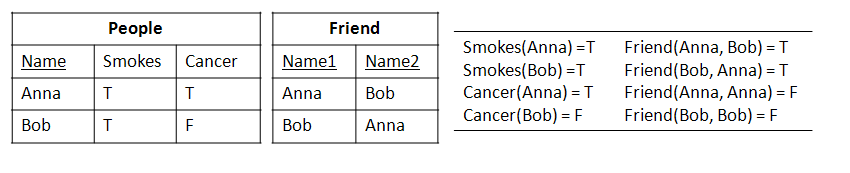
\includegraphics[width = 0.5 \textwidth]{database}
%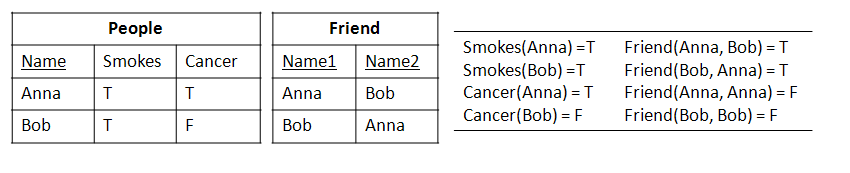
\includegraphics[width=1\textwidth]{database.png}
%}
\caption{A simple relational database instance.
%that are true in the database. 
\label{fig:db-tables}}
\end{center}
\end{figure}


\begin{figure}[t]
\begin{center}
%\resizebox{\textwidth}{!}{
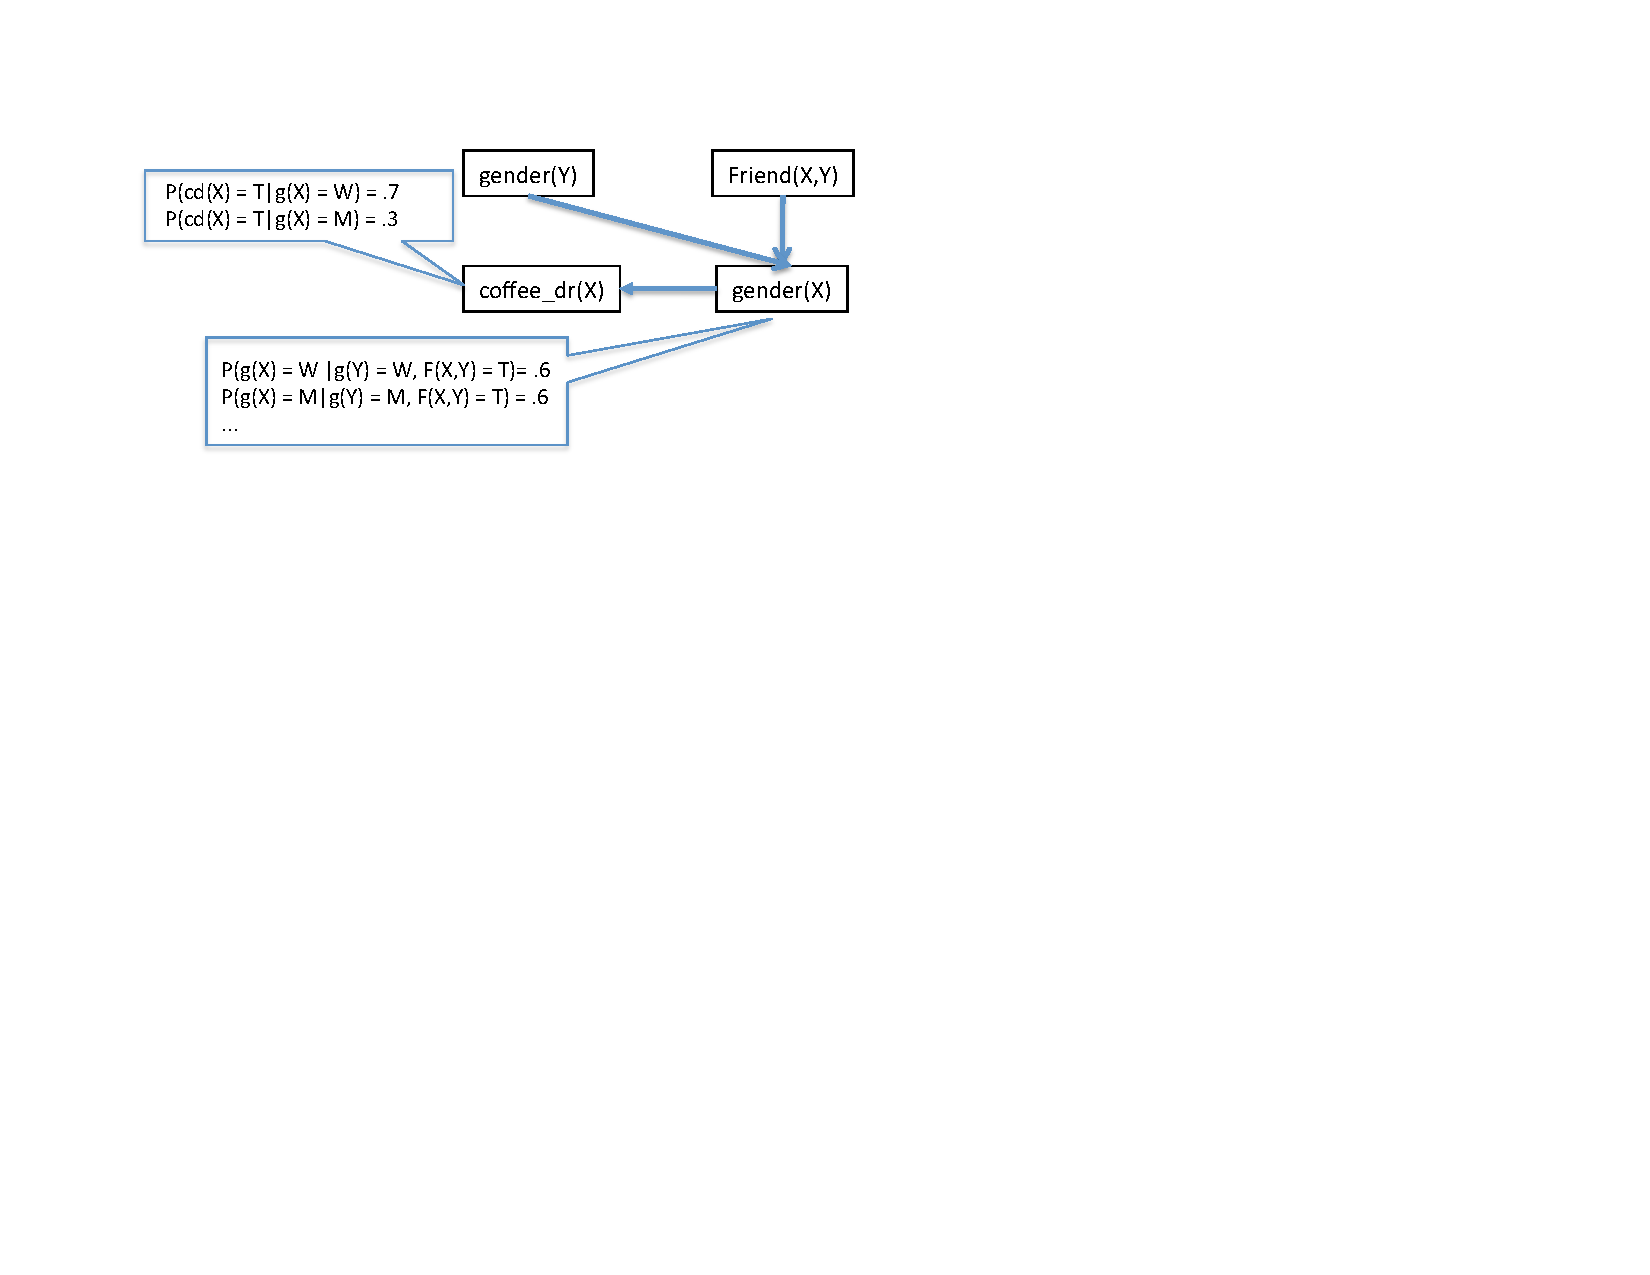
\includegraphics[width = 0.5 \textwidth]{graph-examples}
%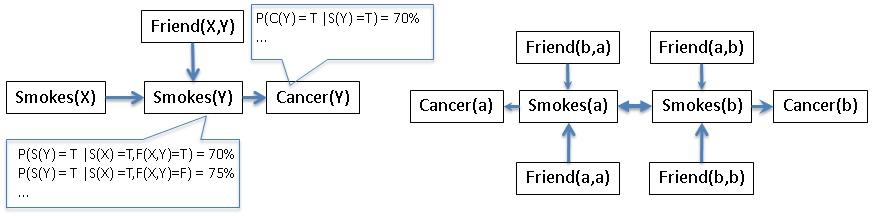
\includegraphics[width=2 \textwidth]{combine1.jpg}
%}
\caption{%A simple relational database instance. 
A Parametrized Bayes Net with some CP-table entries. CP-table entries are chosen for illustration and are not related to the data in Figure~\ref{fig:db-tables}. For convenience, examples below use a uniform prior over the nodes $\it{gender}(\Y)$ and $\it{Friend}(\X,\Y)$.
\label{fig:pbn}}
\end{center}
\end{figure}

%Recursive dependencies (autocorrelations) are represented in a PBN by ``copies'' of the functors. Thus t
%We assume that the Bayes net is in main functor format \cite{Schulte2012a}: for each functor $\functor$, there is a main functor node that is the only $\functor$-node with parents. In the example, $\it{gender}(\X)$ is the main functor, and $\it{gender}(\Y)$ is an auxilliary functor used only for representing the recursive dependency. 
%The intuition is that since different functor nodes with the same functor are statistically interchangeable, it suffices to select one for modelling the conditional distribution. 
%\footnote{While the existence of a main functor may seem like a strong assumption, Schulte {\em et al.} show that under a mild ordering condition on the BN structure, for every PBN $\B$ not in main functor format, there is an equivalent main functor Bayes net $\B'$ that has the same ground graph \cite{Schulte2012a}.}
  
\subsection{Model Conversions.} \label{sec:conversions}
A Bayes net can be converted to a Markov net through the standard \textbf{moralization} method: connect all co-parents, and make all edges in the resulting graph undirected. Thus each family in the Bayes net becomes a clique in the moralized structure. For each state of each family clique, we define the clique potential in the Markov net to be the conditional probability of the child given its parents. 
%This is the conversion procedure recommended by Domingos and Richardson \cite{Domingos2007} and by the Alchemy group \cite{bib:bayes-convert}.
%The resulting Markov net defines the same joint probability over assignments of values to the nodes as the original Bayes net. 
%If $M(\B)$ is a Parametrized Markov net obtained from PBN $B$, the unnormalized likelihood function for the ground graph of $M(\B)$ \cite{Domingos2009} is given by
%
%\begin{equation}\label{eq:mbn-likelihood}
%    P_{\M(\B)}(\set{V} = \set{v}) = exp\left(\sum_{ijk} \instances_{ijk}(\set{V} = \set{v}) \cdot ln(\theta_{ijk})\right).
%\end{equation}

%This is because each ground parent-child instance corresponds to a conditional probability $\theta_{ijk}$, viewed as a clique potential, so 
%Thus the likelihood is proportional to the product of all conditional probabilities. 
%In terms of the Bayes net parameters, Equation~\eqref{eq:mbn-likelihood} is simply the product of all conditional probabilities defined by a ground child-parent instance.
A PBN graph can be converted to a Markov Logic Network structure by moralization \cite[12.5.3]{Domingos2007}, \cite{Schulte2012}: for each family state $\family_{ijk}$, add a conjunction of literals that specifies the state.


Bayes nets can also be converted to dependency nets \cite{Heckerman2000}. For each node $\X_{i}$, and each node  $\X_{j}$ in the Markov blanket of $\X_{i}$, add a directed edge $\X_{j} \rightarrow \X_{i}$. 
%The resulting graph is the same as the moralized Bayes net structure but with bidrected rather than undirected adjacencies. 
The conditional probability parameters are  given by the Markov blanket equation ~\eqref{eq:bn-mb}.

%A \textbf{Markov Logic Network} (MLN) is a finite set of 1st-order formulas or clauses $\{\formula_{i}\}$, where each formula $\formula_{i}$ is assigned a weight. 
%A Markov Logic Network can be viewed as a specification of a Markov network using logical syntax \cite{Domingos2009}. Given an MLN and a database $\D$, let $n_{i}(\D)$ be the number of groundings that satisfy $\formula_{i}$ in $\D$.
%%An MLN assigns a log-likelihood to a database according to the equation
%%
%%\begin{equation}\label{eq:log-linear}
%%ln(P(\D)) = \sum_{i} w_{i} n_{i}(\D) - ln(\Z)
%%\end{equation}
%%where $\Z$ is a normalization constant.
%%
%%Thus the log-likelihood is a weighted sum of the number of groundings for each clause. 
%
%Functor Markov Nets have a simple representation as Markov Logic Networks as follows. For each assignment of values to a clique of functor nodes, add a conjunctive formula to the MLN that specifies that assignment. The weight of this formula is the logarithm of the clique potential. For any Functor Markov net,  the MLN likelihood function defined by Equation~\eqref{eq:log-linear} for the corresponding MLN is exactly the Markov net likelihood defined by grounding the Functor Markov net. {\em Therefore we can use MLN inference to carry out inference for Functor Markov Nets.}

\section{Random Regression} 
%We first define random regression, then provide a closed form for computing its value that leads to the frequency log-linear model. The frequency model is a locally scaled version of the standard count log-linear model that is derived from Markov random fields.
%
%\subsection{Definition of Random Regression}

Let $\Y = \functor(a_{1},\ldots,a_{\l})$ be a target ground node instantiating functor node $\functor(\A_{1},\ldots,\A_{\l})$.
%\footnote{[If there are several nodes with functor $\functor$, we assume that there is only one node with $\functor$ that has parents, and use that node. Schulte {\em et al.} prove that under a mild ordering condition on the BN structure, for every PBN $\B$ there is an equivalent PBN $\B'$ that satisfies the unique node condition and has the same ground graph \cite{Schulte2012a}.]}
The \textbf{regression graph} for $\Y$ is the partially ground PBN %$B_{Y}$ 
that results by substituting $a_{i}$ for $A_{i}$ in functor node $Y$ {\em and} in its Markov blanket; see Figure~\ref{fig:regress}.
%. This is illustrated in Figure~\ref{fig:regress} for the grounding $\X:= \it{sam}$. 
%If there is more than one functor node with $\functor$, we use the main functor node (Sec.~\ref{sec:graph-relational}). 
Given a target node value $\y$ and an assignment $\set{X} = \set{x}$ of values to all ground nodes other than $Y$, random regression is defined by the following steps.
%For an assignment $\set{X} = \set{x}$ of values to all ground nodes other than $Y$, let $\instances_{ijk}(\set{X}=\set{x};\Y=\y)$ be the number of instantiations in the partially ground model that assign value $y$ to $Y$, and whose family state is $\family_{ijk}$. If family $\family_{ijk}$ does not contain functor node $\functor$,  $\instances_{ijk}(\set{X}=\set{x};\Y=\y) = 0$. If the PBN contains more than one node with functor $\functor$, the instances are counted with respect to grounding the main functor node. 

\begin{enumerate}
\item Let $\A_{1},\ldots,\A_{k}$ be a list of {\em all} first-order variables that occur in the Markov blanket of target node $\Y$ in the regression graph for $\Y$.
\item Select an instance (constant) $a_{i}$ from the population of $\A_{i}$, for each $i=1,\ldots,k$; the selections are random, independent, and uniform. Replace each node in the Markov blanket with the corresponding ground node.
\item Using the values assigned to the ground nodes in the database, apply the Bayes net Markov blanket equation~\eqref{eq:bn-mb} 
to compute the factor product for $\Y$; this defines a log-sum for the random instantiation $\set{a_{i}}$. The expected value of this log-sum is the \textbf{random regression} value $ln(\tilde{P}^{r}(\Y = \y|\set{X}=\set{x}))$. 
\end{enumerate}

\begin{figure}
\begin{center}
%\resizebox{1\textwidth}{!}{
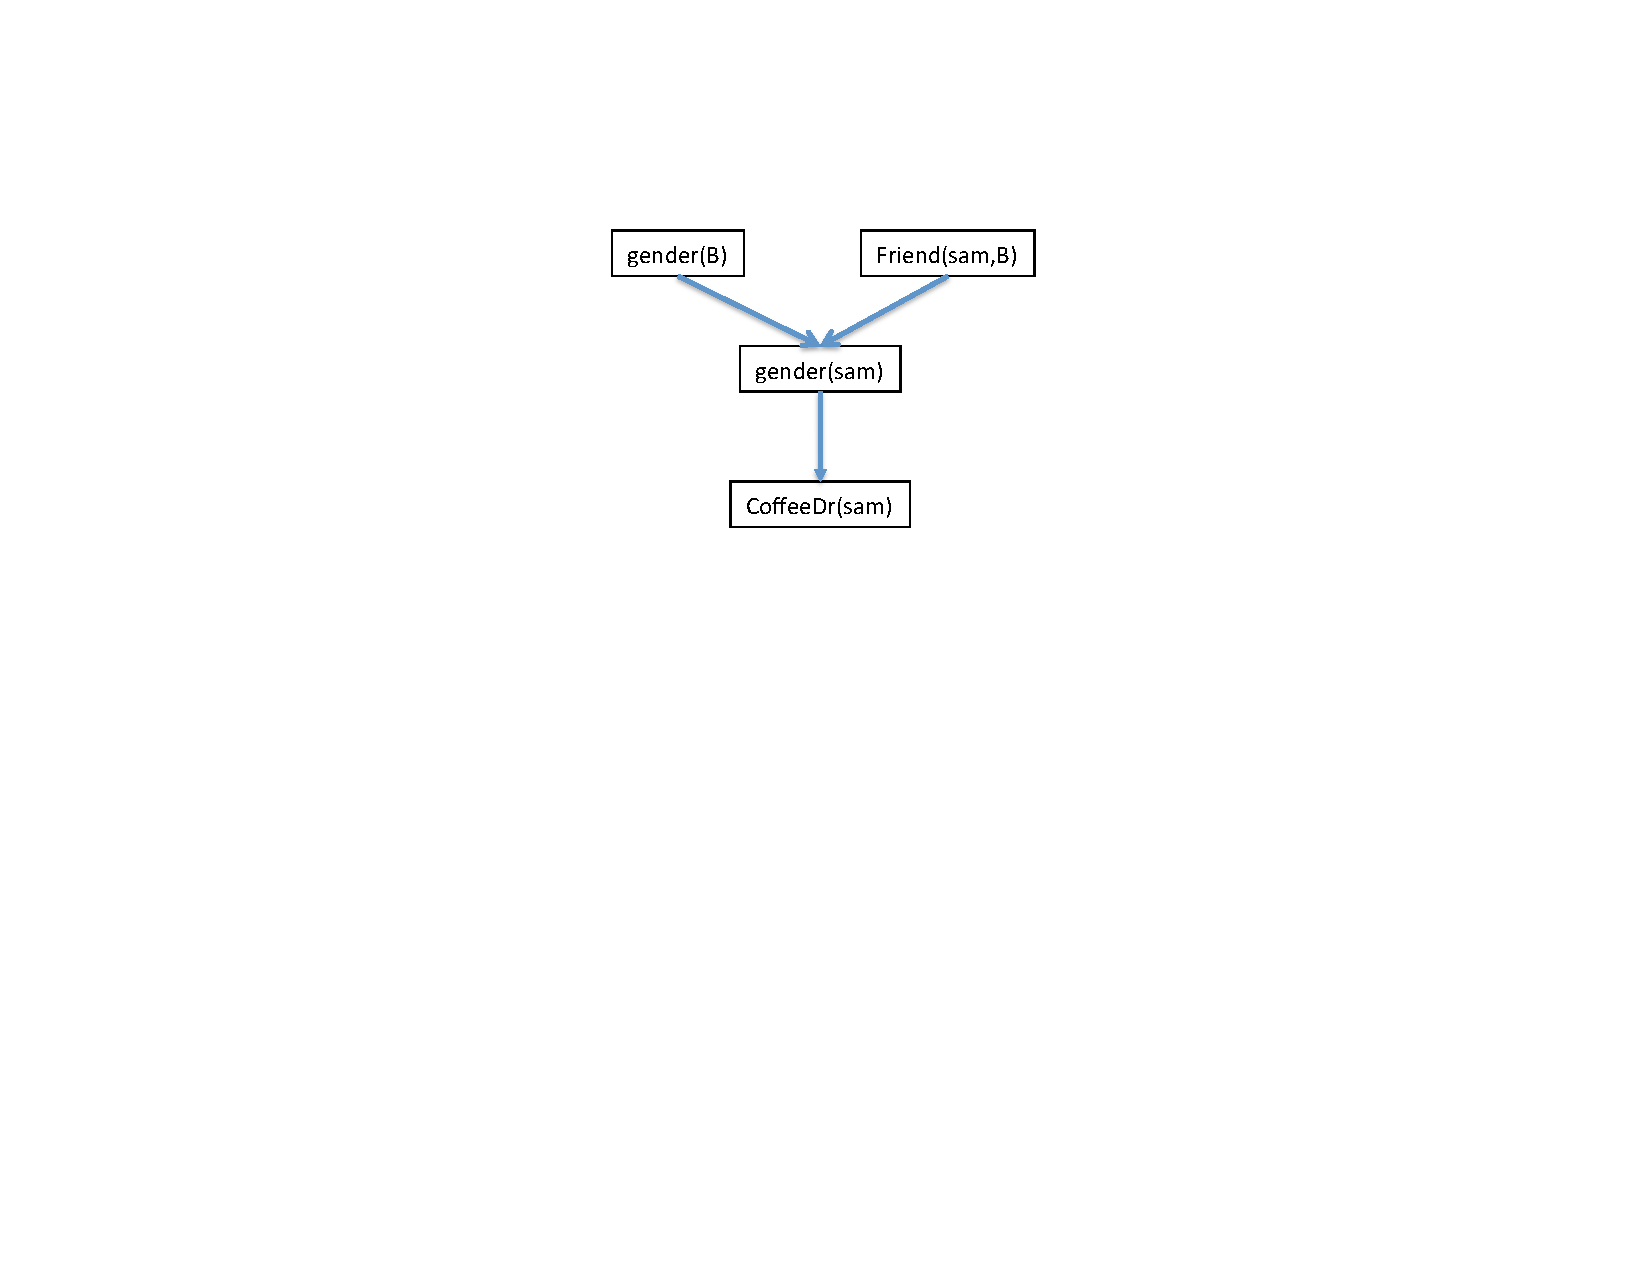
\includegraphics[width =0.4 \textwidth]{regression-graph}
%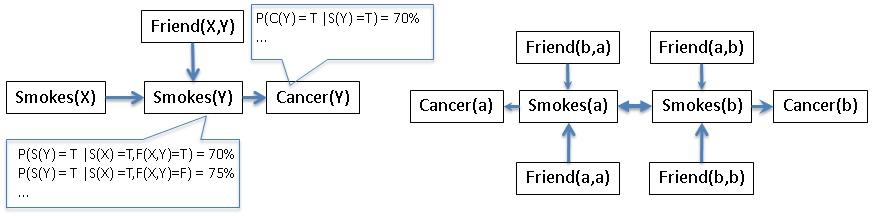
\includegraphics[width=2 \textwidth]{combine1.jpg}
%}
\caption{%A simple relational database instance. 
The regression graph for the target node $\it{gender}(sam)$ derived from the Bayes net of Figure~\ref{fig:pbn} by substituting $sam$ for $\X$.
 \label{fig:regress}}
\end{center}
\end{figure}



Including irrelevant predictors leads to bad predictions, so statistical-relational models restrict edges in the ground model to relevant predictors only \cite{Poole2003}. % add Natarajan on cominbing rules, Getoor and Grant. 
In what follows, we take the relevance conditions to be the existence of a link, {\em so we only consider instances of the Markov blanket that are related to the target node.} Table~\ref{table:random-regress} provides a sample computation of a random regression for predicting the gender of Sam given the database instance of Figure~\ref{fig:db-tables}. 
%The random regression inference model can be interpreted in terms of a ground dependency network, whose graph structure is given by converting the Bayes net to a dependency network (Sec.~\ref{sec:conversions}), and whose conditional probability parameters are given by random regression. 
The next section relates random regression to log-linear models for relational prediction.


\begin{table}[htdp]
\caption{Computing the random regression for target node value $\it{gender}(sam) = W$. We use obvious abbreviations for functors. Each friend selection defines an instantiation of the Markov blanket of the target node with two associated factors. %The random regression value -1.07 is the log-average. 
%Notice that $-1.07=ln(0.34)$, the log of frequency regression (Figure~\ref{fig:regress}).
}
\begin{center}
\resizebox{0.5\textwidth}{!}{
  \begin{tabular}{@{} |c|c|c|c| @{}}
    \hline
  Grounding & Factor 1 & Factor 2 & Log-Product \\
    \hline \hline
   $Y=anna$ & \begin{tabular}{@{} l @{}}
$P(\it{cd}(sam) = T|g(sam) = W)$ \\
= .7\\ \end{tabular} & 
\begin{tabular}{@{} l @{}}
    �$P(g(sam)=W|g(anna) = W, $ \\ 
    � $Fr(sam,anna) = T) = .6$\\ 
  \end{tabular} & 
  \begin{tabular}{@{} l @{}}$ln(.7\times.6)$ \\= -0.87\end{tabular} 
  \\\hline
    Y=bob & \begin{tabular}{@{} l @{}}
$P(\it{cd}(sam) = T|g(sam) = W)$ \\
= .7\\ \end{tabular} & \begin{tabular}{@{} l @{}}
    �$P(g(sam)=W|g(bob) = M, $ \\ 
    � $Fr(sam,bob) = T) = .4$\\ 
  \end{tabular} & 
  \begin{tabular}{@{} l @{}}$ln(.7\times.4)$ \\=-1.27 \end{tabular} 
  \\\hline
  &  & Average & -1.07 \\ \hline
  \end{tabular}
}
\end{center}
\label{table:random-regress}
\end{table}%


%Figure~\ref{fig:regress} illustrates the resulting computation for predicting the intelligence of Bob given the database instance of Figure~\ref{fig:db-tables}.


%For the relevance version, treat each context sentence as having disjoint variables from the others (e.g. R(X,Y), R1(X1,Y1)). Then you get random selections from contexts.

%\begin{table}[htdp]
%\caption{Computing the random regression for target node node value $\it{gender}(sam)$. Each course selection defines an instantiation of the Markov blanket of the target node with two associated factors. The random regression value -1.07 is the log-average. Notice that $-1.07=ln(0.34)$, the log of frequency regression (Figure~\ref{fig:regress}).}
%\begin{center}
%\resizebox{0.5\textwidth}{!}{
%  \begin{tabular}{@{} |c|c|c|c| @{}}
%    \hline
%  Grounding & Factor 1 & Factor 2 & Log-Product \\
%    \hline \hline
%   $C=100$ & \begin{tabular}{@{} l @{}}
%$P(i(bob) = lo|r(bob) = lo)$ \\
%= .7\\ \end{tabular} & 
%\begin{tabular}{@{} l @{}}
%    �$P(i(bob) = lo|diff(100) = lo, $ \\ 
%    � $R(bob,100) = T) = .6$\\ 
%  \end{tabular} & $ln(.7\times.6)$ = -0.87 \\\hline
%    C=200 & \begin{tabular}{@{} l @{}}
%$P(i(bob) = lo|r(bob) = lo)$ \\
%= .7\\ \end{tabular} & \begin{tabular}{@{} l @{}}
%    �$P(i(bob) = lo|diff(200) = hi, $ \\ 
%    � $R(bob,200) = T) = .4$\\ 
%  \end{tabular} & $ln(.7*.4)=-1.27$ \\ \hline
%  &  & Average & -1.07 \\ \hline
%  \end{tabular}
%}
%\end{center}
%\label{table:random-regress}
%\end{table}%

%Grounding & Factor 1 & Factor 2 & Log-Product \\
%C=100 & P(i(bob) = lo|r(bob) = lo) = .7 & P(i(bob) = lo|diff(100) = lo, R(bob,100) = T) = .6 & -0.87 \\
%C=200 & P(i(bob) = lo|r(bob) = lo) = .7 & P(i(bob) = lo|diff(200) = hi, R(bob,200) = T) =.4 & -1.27 \\
% &  & Average & -1.07 \\

\section{Log-linear Relational Regression}

%Recall that 
The general form of a {\em log-linear regression equation} is

$$ln(\tilde{P}(\Y = \y|\set{x}))= \sum_{i} w_{i} x_{i}.
$$
In this section we consider how the predictor variables $x_{i}$ may be derived from a Bayes net. In the next section we examine how the weight parameters $w_{i}$ may be derived from a Bayes net.
%
%Given a Bayes net model, the $x_{i}$ are derived from the states $\family_{ijk}$ of the Markov blanket of target node $y$. 
We consider two specific choices of predictor variables $\{x_{i}\}$. 


\begin{description}
\item[The Frequency Model] The predictor variables $x_{i}$ are the {\em frequencies} $\prob^{\Y}_{ijk}$ of the Markov blanket states for the target node $\Y$.
\item[The Count Model] The predictor variables are the {\em counts} $\instances^{\Y}_{ijk}$ of the Markov blanket states for the target node $\Y$. 
\end{description}

Figure~\ref{fig:regress-example} provides an example computation for frequency regression and for count regression. 

\subsection{Frequency Regression}
If the log-conditional probabilities from the Bayes net CP-table entries are used as weights, then the \textbf{frequency regression equation} is given by



\begin{figure}[t]
\begin{center}
%\resizebox{1\textwidth}{!}{
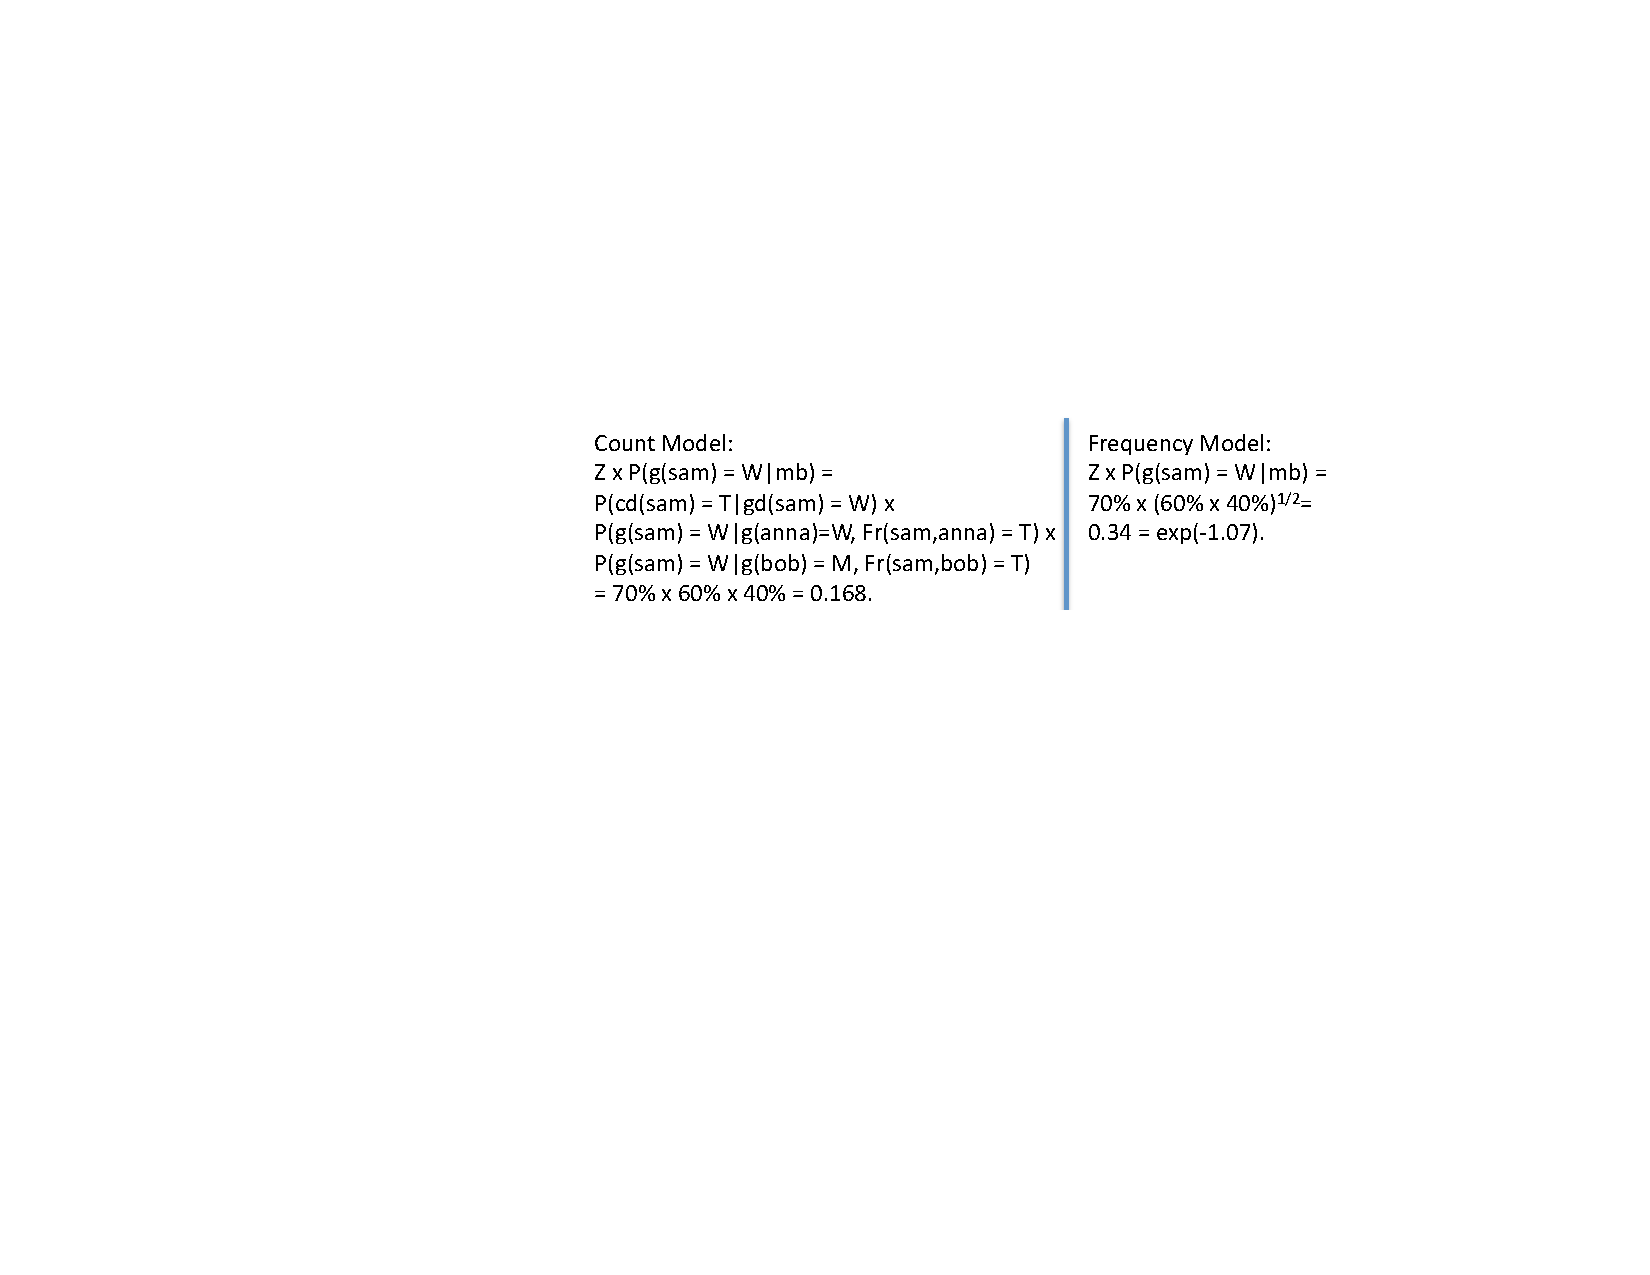
\includegraphics[width=0.5 \textwidth]{regression-example}
%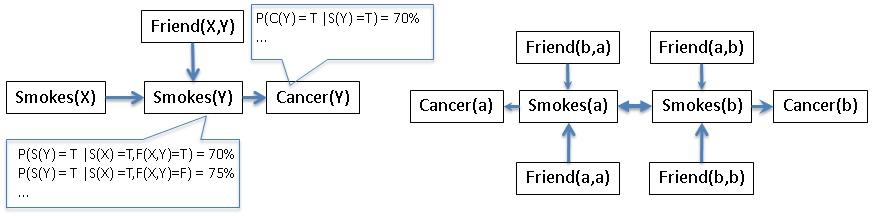
\includegraphics[width=2 \textwidth]{combine1.jpg}
%}
\caption{%A simple relational database instance. 
The computation of the unnormalized Markov blanket probability for the gender of Sam, for the count model (left) and the frequency model (right). 
%The frequency model assigns higher importance to the factor that represents the coffee drinking of Sam. Notice that the log-probability defined by the frequency models agrees with the log-probability defined by random regression.
 \label{fig:regress-example}}
\end{center}
\end{figure}

\begin{equation} \label{eq:regress-frequency}
ln(\tilde{P}(\Y = \y|\set{X}=\set{x})) = \sum_{ijk} p^{\Y}_{ijk}(\set{X}=\set{x},\Y = \y) \; ln(\theta_{ijk}).
\end{equation}

Here and elsewhere the superscript $\Y$ indicates that the notation is used with reference to the regression graph for target node $\Y$. The summation is over $\Y$'s Markov blanket in the regression graph, so the index $i$ ranges over the target node and its children. 
%
For the unnormalized conditional log-likelihood of $\it{gender}(sam) = W$, random regression (Table~\ref{table:random-regress}) gives the same value $0.34 = e^{-1.07}$ as frequency regression.
%, conditional on its Markov blanket. 
The next theorem shows that {\em the  equivalence between frequency and random regression holds in all cases.}  The proof is in the supplementary material. 
\begin{theorem} \label{prop:randomize}
The frequency regression value  for a target node (Equation~\eqref{eq:regress-frequency}) equals the random regression value. 
%; in symbols, $P^{r} = P^{\pseudo}$.
\end{theorem}


%
%Let $m_{iik}^{\Y}$ denote the number of possible groundings of family formula $\family_{ijk}$. 
%%in the regression graph. 
%Here and elsewhere the superscript $\Y$ indicates that the notation is used with reference to the regression graph. If the parents of functor node $i$ contains a relevance condition,   then $m_{ijk}^{\Y}$ denotes the possible number of relevant groundings. For instance, in the regression graph of Figure~\ref{fig:regress}, $m_{ijk}^{\Y}$ with functor node $i$ being $\it{gender}(sam)$, the term $m_{ijk}^{\Y}$ is the number of Sam's friends. 
%Note that $m_{i}$ does not depend on $j$ or $k$. 
%Then the frequency of the family constellation $\family_{ijk}$ is given by dividing the number of satisfying instantiations by $m_{i}$. 


%\begin{equation} \label{eq:regress-frequency}
%\tilde{P}(\Y = \y|\set{X}=\set{x}) = exp\left(\sum_{ijk} \frac{\instances_{ijk}(\set{X}=\set{x},\Y = \y)}{m_{i}} \cdot ln(\theta_{ijk})\right).
%\end{equation}

%\begin{equation} \label{eq:regress-frequency}
%ln(\tilde{P}(\Y = \y|\set{X}=\set{x})) = \sum_{ijk} \frac{\instances^{\Y}_{ijk}(\set{X}=\set{x},\Y = \y)}{m_{ijk}^{\Y}} ln(\theta_{ijk}).
%\end{equation}



%where $\tilde{P}(\Y = \y|\set{X}=\set{x}))$ is the unnormalized probability of a target node value $\Y = \y$ given an assignment of values to all other nodes. 

%The fraction $\instances^{\Y}_{ijk}/m_{ijk}^{\Y}$ is the number of relevant groundings that satisfy family formula $\family_{ijk}$, divided by the total number of relevant groundings, and therefore represents the frequency of family state $\family_{ijk}$ in the set of relevant groundings.
%that avoids an enumeration of all possible groundings of the Markov blanket.

%
%While random regression sums over all groundings of the Markov blanket, frequency regression sums over the {\em non-ground} functor nodes in the Markov blanket. Thus frequency regression provides an efficient closed-form for computing the random regression value.
%We remark that the equivalence between random and frequency regression holds with any graphical model based on a first-order template, not only Bayes nets. 
%Frequency regression can be interpreted in terms of a dependency network that results from grounding a PBN model: The use of frequency predictors is equivalent to using the {\em geometric mean} to combine conditional probabilities in the Markov blanket of the target node, as Figure~\ref{fig:regress} illustrates.


\subsection{Count Regression} \label{sec:count}
 differs from frequency regression in that it uses the family counts $\instances_{ijk}$ rather than the family frequencies $p_{ijk}$. The \textbf{count regression equation} is therefore given by 

\begin{equation} \label{eq:regress-count}
ln(\tilde{P}(\Y = \y|\set{X}=\set{x})) = \sum_{ijk} \instances^{\Y}_{ijk}(\set{X}=\set{x},\Y = \y) \; ln(\theta_{ijk}).\end{equation}

%Since Equation~\ref{eq:regress-count} uses the family counts $\instances_{ijk}$ rather than the family frequencies $p_{ijk}$, we refer to it as the \textbf{count equation}. 
The count equation is closely related to Markov random fields, as follows. Consider the Parametrized Markov net $M$ obtained by moralizing the PBN (Sec.~\ref{sec:conversions}). The count equation follows from applying the standard Markov field regression equation to the grounding of $M$ \cite{Domingos2007}. 
%In graphical terms, the equation is the product of all clique potentials in which the target node participates; see Figure~\ref{fig:regress-example}. 
%Count regression is a natural comparison point to random regression due to their similarity. 
%
%In the count regression equation~\eqref{eq:regress-count}, Markov blanket components with many groundings have exponentially more influence. 
%In a typical scenario, a descriptive attribute of a target entity corresponds to a single factor, whereas the attributes of related entities correspond to many, as many as there are related entities. For example, in the prediction of intelligence in Figure~\ref{fig:regress}, the factors due to courses quickly overwhelm the influence of rank as the number of courses increases. 
%The frequency model balances the scales of the predictor variables, such that their common range is [0,1]. 
In terms of the factor products defined by exponentiating the log-linear equations, the two models compare as follows. The count equation multiplies together all ground Markov blanket factors, whereas the frequency equation first computes the {\em geometric mean} of the ground factors associated with each functor node in the Markov blanket, then multiplies these geometric means (Figure~\ref{fig:regress-example}). Both regression models can be interpreted in terms of a dependency network that results from grounding a PBN model.
Figure~\ref{fig:derivations} summarizes the connections between graphical models and regression equations. In the next section we consider how to derive the weight parameters from given Bayes net parameters.

\begin{figure}[htbp]
\begin{center}
%\resizebox{0.5\textwidth}{!}{
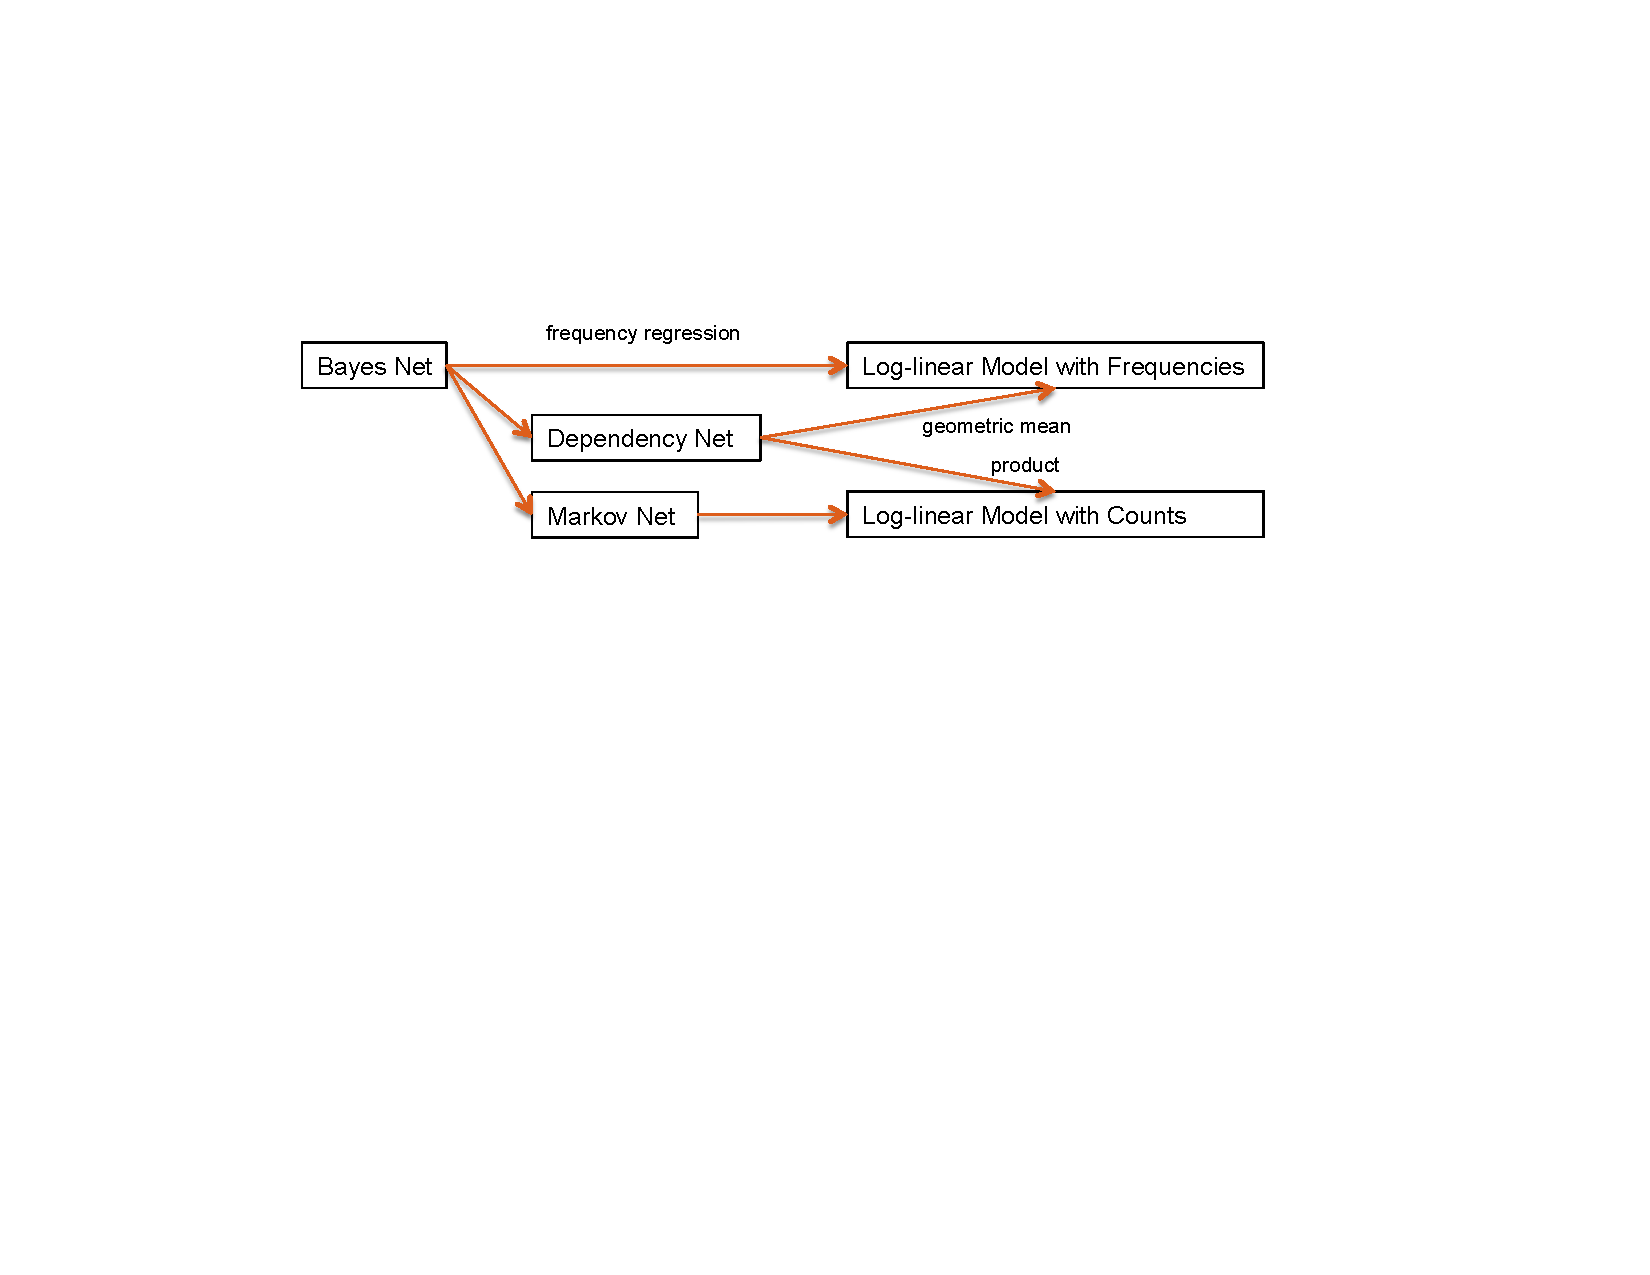
\includegraphics[width = 0.5 \textwidth]{derivations}
%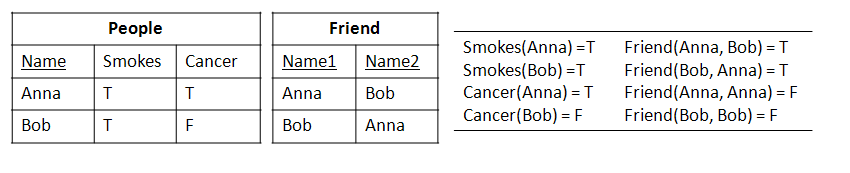
\includegraphics[width=1\textwidth]{database.png}
%}
\caption{Connections between graphical models and log-linear regression equations. 
%Applying random regression directly to a PBN leads to the frequency model (Theorem~\ref{prop:randomize}). Converting the Bayes net to a Markov net leads to the count model. Converting the Bayes net to a dependency network leads to the frequency model if the geometric mean is used to combine Markov blanket conditional probabilities. Using the product of conditional probabilities instead leads to the count model. 
\label{fig:derivations}}
\end{center}
\end{figure}



%\paragraph{Inference.} 
%Assuming complete data, the regression equations can be evaluated in closed-form for conditional inference. We outline how the regression models can be extended to general joint inferences. For the count model, Markov logic network inference algorithms can be used after moralization, as in \cite{Khosravi2012a,Schulte2012}. 
%Heckerman et al. \cite{Heckerman2000} show that applying Gibbs sampling to a dependency network defines a stationary joint distribution, hence can be used to answer general queries based on random/frequency regression. Their ordered pseudo-Gibbs sampler has been lifted to the relational setting \cite{Neville2007}. 
%%A Gibbs sampler for random regression would be able to exploit the ordering constraints provided by the Bayes net structure. 
%Since the form of the frequency equation is very similar to that of the count model, an alternative is to adapt MLN inference methods developed for the count model.
%
%So far we have considered how to derive the predictor variables $x_{i}$ from a given Bayes net graph. 




\section{Weight Learning With Bayes Net Parameters}

For estimating the conditional probabilities, we use the empirical conditional frequencies observed in the database:

\begin{equation*} \label{eq:frequencies}
\widehat{\theta}_{ijk}(\set{V} = \set{v}) = \frac{n^{\Y}_{ijk}(\set{V} = \set{v})}{\sum_{k}n^{\Y}_{ijk}(\set{V} = \set{v})}.
\end{equation*}

These estimates are well motivated by the following theoretical and practical considerations. 
%\marginpar{check Poole}

\emph{Maximum Likelihood.} The  random selection pseudo-likelihood for a Bayes net is the natural generative counterpart of random regression \cite{Schulte2011}. This measure is the expected log-likelihood of a random instantiation of all first-order variables in the Bayes net. The pseudo-likelihood is maximized by the conditional frequencies $\widehat{\theta}_{ijk}$ in the database \cite[Prop.3.1]{Schulte2011}. 
%This result is a counterpart to the standard maximum likelihood solution for i.i.d. propositional data.

\emph{Interpretability.} The weight/clique potential parameters of undirected models are often difficult to interpret for users \cite{Pearl1988}. 
This is especially the case when weights are learned from data, with complex interactions between weights assigned to different local cliques. In contrast, a Bayes net parameter can be interpreted as a conditional probability, and reflects local statistics restricted to a parent-child constellation.

\emph{Scalability.} 
Using frequency estimates can be viewed as a type of {\em lifted learning}, by which we mean using only the sufficient statistics in a relational database, rather than an iteration over ground facts. The computational cost of lifted learning scales well in both data size and the number of parameters in the model. 

We investigate two methods for converting Bayes net conditional probabilities to log-linear weights $w_{ijk}$. 

\subsection{Log-conditional Probabilities as Weights.} \label{sec:logprob} The first method uses the logarithm of the conditional probability of a child node value given values for its parents. In symbols:

\begin{equation*}
w_{ijk} := ln(\theta_{ijk}).
\end{equation*}

{\em Example.} As in Section~\ref{sec:graph-relational}, consider the family state 
$\family_{ijk}$ with $\theta_{ijk} = 40\%$. In the Markov Logic network that results from converting the PBN, this parameter leads to the weighted conjunctive clause 
\[g(\X)= M, g(\Y) = W, F(\X,\Y) = \true; w = ln(40\%).\]% = -0.916. \]

Other researchers have recommended log-conditional probabilities as weights   \cite{Domingos2007}, \cite{bib:bayes-convert}. 
%In the propositional case, if we convert a Bayes net to a Markov net by moralization and use the log-conditional probabilities as weights (logarithm of clique potentials), then the joint distribution defined by the Bayes net is equivalent to the joint distribution defined by the Markov net \cite{Lauritzen1996}. 

{\em The Scale Problem.} 
A problem with using log-conditional probabilities together with the count model is that features with more instances have exponentially more influence; see Figure~\ref{fig:regress-example}. In a typical illustrative scenario, the regression target is the descriptive attribute of a single entity, (e.g., $\it{gender}(sam)$). One predictor feature represents an association between attributes of the same entity (e.g., $\it{coffee\_dr}(sam),\it{gender}(sam)$, whereas another represents an association between attributes of related entities and the single entity (e.g., $\it{gender}(sam), \it{gender}(\Y),\it{Friend}(\it{sam},\Y) = \true$). In this case the information from related entities has many instances, and tends to overwhelm that from the target entity, which has just one instance. In terms of a log-linear model, the count predictors are on different scales. 
%In a general log-linear model, the weights can be adjusted so that predictors with large values receive smaller weights. But 
%since in a Bayes net model, the weights are on the same scale (log-probability), log-conditional probabilities do not sufficiently scale down the impact of predictors with larger grounding counts. 
{\em Frequency regression balances the impact of different features by scaling predictors to the common range [0,1].}  
%Our second conversion procedure also addresses the scale problem,  by adjusting the weights. % derived from log-conditional probabilities.

\subsection{Log-differences as Weights.} \label{sec:log-diff}
The second method uses the log-difference between the conditional probability of a child node value given values for its parents, and the prior unconditional probability of the child node value. 
%Recall from Section~\ref{sec:graph-relational} that the notation $\family_{i0k}$ refers to node $i$ taking on value $k$ without any specification of parent values, with the corresponding interpretation of $\instances_{i0k}$ and $\prob_{i0k}$.
%of the Bayes net parameters as weights. To define this formally, let us first write $\instances_{i0k}(\set{V} = \set{v})$ for the number of groundings of child node $\Y$ such that the ground node $\y$ is assigned value $k$, and similarly $p_{i0k}(\set{V} = \set{v})$ for the frequency of such groundings. 
A Bayes net implicitly defines a value $\theta_{i0k}$ for the marginal probability of node $\X_{i}$ taking on value $k$, which can be computed using a standard Bayes net query (or directly estimated from the data).
%If we use maximum likelihood estimation, the empirical frequency of functor node $i$ taking on value $k$ is given by
%
%\[\widehat{\theta}_{i0k}(\set{V} = \set{v}) = \frac{\instances_{i0k}(\set{V} = \set{v})}{\sum_{k} \instances_{i0k}(\set{V} = \set{v})}.\]
%
The log-difference weight assignment is 
\begin{equation*}
w_{ijk} := ln(\theta_{ijk}) - ln(\theta_{i0k}).
\end{equation*}

%This method requires adding the predictor variable $\instances^{\Y}_{i0k}$ to the count equation~\ref{eq:regress-count}, and the predictor variable $p_{i0k}$ to the frequency equation~\ref{eq:regress-frequency}. In either case, the weight of the new predictor variable is $w_{i0k}$.
% When discussing the log-difference model, we assume  implicitly that these predictors have been added to the model. In terms of 
%%Markov random fields, the predictor variables correspond to a potential for a singleton clique; in terms of 
%Markov Logic Networks, they correspond to adding unit clauses. 
%
{\em Example.} For the Bayes net of Figure~\ref{fig:pbn}, assume that conditional on $\X$ and $\Y$ {\em not} being friends, the distribution of $g(\X)$ is  uniform regardless of the value of $g(\Y)$. For instance, $P(g(\X)=W|F(\X,\Y) = F, g(\Y) = M) = 1/2$. Then the marginal probability distribution that the Bayes net entails for $g(\X)$ is also uniform, that is, $P(g(\X) = M) = P(g(\X) = W) = 50\%.$
%
For each marginal probability assignment, the Markov Logic network that results from converting the PBN contains a unit clause with weight the log-marginal probability. In the example, there is a weighted clause \[g(\X) = M; w = ln(50\%). \]
%= -0.693.\] 
For each family state $\family_{ijk}$, the MLN contains a conjunctive clause, with the weight being the log-difference between the conditional and the marginal probabilities. In the example, there is a weighted clause 

\begin{small}
\[g(\X)= M, g(\Y) = W, F(\X,\Y) = \true; w = ln(40\%) - ln(50\%).\]
% = -0.223.\]
\end{small}
{\em Motivation and Discussion.} 
%One advantage of the log-difference method is that the weights can be interpreted in terms of relevance, as usual in a linear model. Thus a positive weight means positive relevance: the parent condition lifts the probability of a child node value, a negative weight means negative relevance: the parent condition lowers the probability of a child node value, and a 0 weight means irrelevance: the parent condition does not affect the probability of a child node value.
%
%Our main motivation for the log-difference method is to improve predictions by addressing the scale problem. 
%For a child node that refers to a descriptive attribute of a single entity, (e.g., $\it{gender}(\X)$), formulas with many groundings are those that express an association between attributes of related entities and the single entity (e.g., the formula $\it{gender}(\Y) = W, \it{gender}(\X)= M,\it{Friend}(\X,\Y) = \true$ introduces a connection between the gender of a user and that of his or her friends). 
The reason why log-difference addresses the scale problem is as follows.
Compared to associations among the attributes of a single entity, we expect the associations with related entities to be relatively weak, because probabilistic dependencies in a network become weaker with distance. This means that the probability of a child value, given a parent condition specifying descriptive attributes of related entities, should be relatively close to the marginal probabilities of the child value. Therefore the log-difference should be relatively small, and so the log-difference method tends to assign smaller weights to formulas with many groundings. The supplementary material confirms this expectation with direct observations of the weight sizes assigned to different formulas. It also shows that weights found by Markov field optimization methods are smaller for formulas with many groundings, which is further evidence that a scaling component is important for weights in the count model.

%In the next section we present empirical observations that compare the balancing effect of the log-difference and other weight learning methods.

%

%While using the frequency model is the most direct and effective way to address the scale problem, the log-difference method is useful if the goal is to use a count-based model of inference, such as a Markov Logic Network.
%We evaluate different weight learning methods in two ways: i) by considering how they scale weights, and ii) by the predictive performance of the resulting models. 
%
Our final section evaluates the different methods on learning time and predictive accuracy.

\section{Performance Evaluation}

We first discuss our comparison metrics, then the systems compared. All experiments were done on a QUAD CPU Q6700 with a 2.66GHz CPU and 8GB of RAM. Our code and datasets are available on the world-wide web \cite{bib:jbnsite}. 

% and the comparison results.
%\subsection{Datasets}

\subsection{Performance Metrics.}
We use 3 performance metrics: %measures: goo	ggg
Learning Time, Accuracy (ACC), and Conditional Log Likelihood (CLL). ACC and CLL have been used in previous studies of MLN learning  \cite{Domingos2007,Schulte2012}. The CLL of a ground atom in a database is given by the log of the regression equation. For a database we report the average CLL over all atoms in the test set. To define accuracy, we apply inference to predict the probability of an attribute value, and score the prediction as correct if the most probable value is the true one. For ACC and CLL the values we report are averages over all predicates that represent descriptive attributes.
%We do not use Area Under Curve(AUC) as it is mostly used for binary predicates.
%The AUC curves were computed by changing the CLL threshold above which a ground atom is predicted true (10 thresholds were used).
We do not use Area Under Curve, as it mainly applies to binary values, and most of the attributes in our dataset are nonbinary. 
%Like previous studies, we used the MC-SAT inference algorithm \cite{Poon2006} to compute a probability estimate for each possible value of a descriptive attribute for a given object or tuple of objects.  %In principle, our 
We evaluate the learning methods using 5-fold cross-validation as follows. We formed 5 subdatabases for each database, by randomly selecting entities from each entity table, and restricting the relationship tuples in each subdatabase to those that involve only the selected entities  (i.e., subgraph sampling \cite{Frank1977,Schulte2012}). The models were trained on 4 of the 5 subdatabases, then tested on the remaining fold. We report the  average score over the 5 runs, one for each fold. 

\subsection{Comparison Methods.}

\subsubsection{Structure Learning.} To obtain a Bayes net structure, we applied the learn-and-join algorithm to each database %, which is the start of the art structure learning algorithm for Parametrized Bayes Nets 
\cite{Schulte2012}. 
We then convert the PBN graph to a Markov Logic Network structure (see Section~\ref{sec:conversions}),
%which adds a conjunctive clause for each family state $\family_{ijk}$ (Section). 
declaring attribute predicates as functional, as recommended by the Alchemy Group \cite{bib:bayes-convert}. A limitation of the current learn-and-join algorithm is that it learns a generative model over attributes given link structure, so our evaluation considers only queries that target attributes, not links, following \cite{Khosravi2010,Schulte2012}. 

\subsubsection{Parameter Learning.} 
\paragraph{Bayes Net Methods.}
Pairing the two Bayes net weight types with the two predictor types yields 4 different log-linear regression models. Table~\ref{table:methods} displays the pairings, with names for future reference.\footnote{Khosravi proposed subtracting the logarithm of the uniform distribution from the conditional probability \cite{Khosravi2012b}.
 %(i.e., $ln(1/l)$ for a child node with $l$ possible values)  
 This method is not theoretically equivalent to random regression. We found that using the marginal probabilities $\theta_{i0k}$ performs better than the uniform distribution on both accuracy and log-likelihood. Thus the marginal probabilities appear to be preferable both in terms of theoretical justification and in terms of predictive performance.} 
%
The next proposition shows that {\em for the frequency model},   the log-conditional and the log-difference weights are equivalent. 
This result means that the extent to which the log-difference method addresses the scaling problem, is already built into the frequency model.
%Basically, the reason is that the log-linear sum contains a sum of the log-marginal, weighted by probabilities. Since the probabilities add up to 1, the log-marginal from adding the unit clauses cancels out the log-marginal term in the log-differences. %In the case of 0 groundings for  target entity, use the prior probability.

\begin{table}[t]
\caption{Regression models + Bayes net weight conversion methods; the frequency models are mathematically equivalent to each other and to random regression.}
\begin{center}
\resizebox{0.5\textwidth}{!}{
\begin{tabular}{|c|c|c|}
\hline Weights/Predictors & Count & Frequency \\\hline
Log-conditional probabilities & log(cp)+count & log(cp)+freq \\\hline
Log-differences & log-diff+count & --- \\\hline
\end{tabular}
}
\end{center}
\label{table:methods}
\end{table}%


\begin{proposition}
Frequency regression (Equation~\ref{eq:regress-frequency}) returns the same result for log-conditional probability weights and for log-difference weights.
\end{proposition}



% KEEP THIS: if we restrict to relevant relations, we can do the same proof conditional on the existence of a relationship. the only issue is if there are 0 groundings for all applicable formulas. In this case it's better to use log-diff, i.e., the true prior, rather than the uniform one.



%Parameter learning for general weights proceeds in two steps as in \cite{Schulte2012}: (1)  %A \textbf{Markov Logic Network} (MLN) is a finite set of 1st-order formulas or clauses $\{\formula_{i}\}$, where each formula $\formula_{i}$ is assigned a weight. A Markov Logic Network can be viewed as a specification of a Markov network using logical syntax \cite{Domingos2009}. 
%Parametrized Markov Nets have a simple representation as Markov Logic Networks as follows. For each assignment of values to a clique of functor nodes, add a conjunctive formula to the MLN that specifies that assignment. The weight of this formula is the logarithm of the clique potential. By converting PMNs to MLNs, we can use MLN inference to carry out inference for PMNs.
%

\paragraph{Markov Net Methods.}

A Markov net model uses general weights $w_{ijk}$.
%in place of $ln(\theta_{ijk})$ derived from a conditional probability. 
To learn the $w_{ijk}$ weights, we applied the default weight training procedure \cite{Lowd2007} of the Alchemy package \cite{Kok2009a}. (We added unit clauses for each node-value combination (cf. Section~\ref{sec:log-diff}), as recommended by the Alchemy group.)  We refer to this method as the \textbf{MBN} method, for ``Moralized Bayes Net''   \cite{Khosravi2010}. 
MBN is the state-of-the-art method for log-linear prediction with Bayes nets \cite{Schulte2012}.
%, and therefore our baseline comparison. 
%For the other methods, i

\subsubsection{Inference}
is performed by evaluating the count resp. frequency regression equation. We employ exact inference rather than approximate inference (e.g., MC-SAT) to avoid conflating the impact of the inference model with the impact of the inference implementation. We conducted experiments with MC-SAT and the results were similar. For MBN we use the count inference model because Alchemy weight learning is optimized for this.
%\footnote{We also experimented with MBN+ the frequency model, with very similar performance to the count model.} 

%
%We compared the following approaches.
%
%
%%\textbf{MLN+ MLN}: We use Alchemy's default program (version x) for producing a parametrized Markov network.
%
%\begin{description}
%\item[MBN] As described above, the Bayes net structure is converted to an MLN using moralization, 
%%\item[MBN+Frequency] Same as the previous method, but using frequency regression for inference. 
%%Alchemy optimizes weights for the count model; we include this method to assess the impact of frequency scaling for weights other than log-conditional probabilities.
%
%\item[CP+Count]  Parametrizes the Bayes net with the empirical conditional probabilities and uses count regression.
%% Actually, this is using the linear shift, or log-difference method.
%\item[CP+Frequency]  Parametrizes the Bayes net with the empirical conditional probabilities and uses frequency regression.
%\end{description}


\subsection{Databases.}

We used %one synthetic and 
5 benchmark real-world databases.   
%The databases are fairly complex, so the experiments are computationally demanding, especially the Alchemy inference component, which needs to be applied to all groundings of all descriptive attributes to compute average predictive performance. The databases and their main characteristics are as follows. 
For more details please see the references in \cite{Schulte2012} and on-line sources such as \cite{bib:jbnsite}.
%In this paper we report the average result over all subdatabases in this paper and leave the evaluation of how models should evolve based on the size of data to an extension of the work in a journal paper. 


%{\em University Database.} We manually created a small dataset, based on the schema given in Table~\ref{table:university-schema}.
%The dataset is small and is used as a toy example for testing purposes. There are three entity tables, Student, Course, Professor, and 2 relationship tables RA and Registered.
%The entity tables contain 38 students, 10 courses, and 6  Professors. The $\reg$ table has 92 rows and the $\it{RA}$ table has 25 rows. %This dataset is translated into 513 ground atoms.

{\em MovieLens Database.} This is a standard dataset from the UC Irvine machine learning repository. 
% \cite{Schulte2012}.
%The schema for the dataset is shown in Table \ref{}.
%It contains two entity tables: $\it{User}$ and with 941 tuples and $\it{Item}$ with 1,682 tuples, and one relationship table $\it{Rated}$ with 80,000 ratings. The $\it{User}$ table has key field $\it{user\_id}$ and 3 descriptive attributes $\age, \it{gender}, \it{occupation}$. We discretized the attribute age into three bins with equal frequency. The table $\it{Item}$ represents information about the movies. It has 17 Boolean attributes that indicate the genres of a given movie. We performed a preliminary data analysis and omitted genres that have only weak correlations with the rating or user attributes, leaving a total of three genres.
%
%The full dataset contains 170,143 ground atoms and is too big for Alchemy to perform learning. We made small subsamples to make the experiments feasible. Subsampling 100 Users and 100 Items transforms to an Alchemy input file with 3,485 ground atoms. Structure learning with Alchemy takes around 30 min.
%Subsampling 300 Users and 300 Items transforms to an Alchemy input file with 27,134 ground atoms. Structure learning with Alchemy takes about 2 days to run.
%The full table with 100,000 ratings exceeded the memory limits of Tetrad, so we randomly picked 40\% of the ratings of the relationship table as input data.

{\em Mutagenesis Database.} This dataset is widely used in ILP research.
% \cite{Srinivasan1996}. %It contains 4 tables total to 15218 tuples. 
It contains information on Atoms, Molecules, and Bonds between them. We use the discretization of \cite{Schulte2012}.
%
%Mutagenesis has two entity tables, $\it{Atom}$ with 3 descriptive attributes, and $\it{Mole}$, with 188 entries and 5 descriptive attributes, including two attributes that are discretized into ten values each (logp and lumo).
%% There are two relationships $\it{MoleAtom}$ indicating which atoms are parts of which molecules, and $\it{Bond}$ which relates two atoms and has 1 descriptive attribute. 
%The full dataset, with 35,973 ground atoms, crashed Alchemy with both structure  and parameter learning. A subsample with 5,017 ground atoms did not terminate for structure learning, but weight learning was feasible. The computational difficulties of Alchemy compared to the MovieLens dataset are  due to the high number of descriptive attributes.
%%another subsample with
%Representing a relationship between entities from the same table in a parametrized Bayes net requires using two or more variables associated with the same population (e.g., $\it{Bond}(\A_{1},\A_{2}))$.
%(Techreport 2009) describes a straightforward extension of Algorithm~\ref{alg:structure} for this case, which we applied to the Mutagenesis dataset.\footnote{Reference omitted for blind review.}
%We also tested our method on the Financial dataset with similar results, but omit a discussion due to space constraints.

{\em Hepatitis Database.} This data is a modified version of the PKDD�02 Discovery Challenge database.
% \cite{Frank2007}. %, which includes removing tests with null values. 
The database contains information on the laboratory examinations of hepatitis B and C infected patients. 
%The examinations were realized between 1982 and 2001 on 771 patients. The data are organized in 7 tables (4 entity tables,  3 relationship tables and 16 descriptive attributes). They contain basic information about the patients, results of biopsy, information on interferon therapy, results of out-hospital examinations, results of in-hospital examinations. 


{\em Mondial Database.} 
%
%\textbf{Hassan: which version did you use? The full one from http://www.dbis.informatik.uni-goettingen.de/Mondial/mondial-ER.pdf or Bahareh's?} 
%
This dataset contains data from multiple geographical web data sources. %Our dataset contains 4 entity tables, $\it{Country},\it{Continent},\it{Economy},\it{Government}$, where the latter three are related to Country by many-one relationships, and one relationship table $\it{Borders}$ that relates two countries.

%Table~\ref{table:datasetsize} lists the resulting full database  sizes in terms of total number of tuples and number of ground atoms, which is the input format for Alchemy. 
%\begin{table}[thbp] \centering
%%\scalebox{0.9}{
%\begin{tabular}[c]
%{|l|l|l|}\hline
% \textbf{Dataset} & \textbf{\#tuples} & \textbf{\#Ground atoms} \\\hline
%%University&171&513\\\hline
%Movielens &82623&170143\\\hline
%Mutagenesis &15218& 35973 \\\hline
%Hepatitis &12447&71597 \\\hline
%%Financial&&\\\hline
%Mondial & 814 & 3366\\\hline
%\end{tabular}
%%} % end scalebox
%\caption{Size of full datasets in total number of table tuples and ground atoms. Each descriptive attribute is represented as a separate function, so the number of ground atoms is larger than that of tuples.\label{table:datasetsize}}
%\end{table}

%\vspace{-10mm}

\emph{UW-CSE database.} This dataset lists facts about the Department of Computer Science and Engineering at the University of Washington (UW-CSE), such as entities (e.g., Student, Professor) and their relationships (i.e. AdvisedBy, Publication).
% \cite{Domingos2007}. 
%The total number of ground atoms is 4,106,841. The database contained a total of 3380 ground atoms. 
The dataset was obtained  by crawling pages in the department's Web site (www.cs.washington.edu). 
%Publications and AuthorOf relations were extracted from the BibServ database (www.bibserv.org). 


\subsection{Results.}

All results are averages from 5-fold cross validation, over all descriptive attributes in the database. 

\subsubsection{Learning Times.}
Table~\ref{table:learn-times} shows runtime results for parameter learning. We see {\em clear scalability advantages for the maximum likelihood conditional probability estimates}: they take seconds to compute, whereas the local search method requires as much as 10 hours in the worst case (Hepatitis).

\begin{table}[t]
\caption{A comparison of {\em runtime} (seconds) required for parameter learning with a fixed Bayes net structure. 
%The Bayes net methods use the observed conditional frequencies. The Markov net methods use Alchemy's default weight learning. 
Database sizes are specified by the number of tuples and the number of ground atoms. 
%For the Markov net methods, the number of model parameters determines runtime more strongly than datasize.
}
\begin{center}
\begin{large}
\resizebox{0.5\textwidth}{!}{
\begin{tabular}{|c|c|c|c|c|c|}
\hline
Dataset & Bayes Net (s) & Markov Net (s)&\#tuples & \#Ground atoms &\#Parameters \\\hline
UW & \bf{2} & 5 &709&2673 & 125 \\
Mondial & \bf{3} & 90 & 814 & 3366 & %2470 
575\\
MovieLens & \bf{8} & 10800 &82623&170143 &327\\
Mutagenesis & \bf{3} & 14400 &15218& 35973 &880\\
Hepatitis & \bf{3} & 36000 &12447&71597 & 793\\\hline
\end{tabular}
}
\end{large}
\end{center}
\label{table:learn-times}
\end{table}%
%UW values are from Zhensong
\subsubsection{Predictive Accuracy.} Table~\ref{table:cll} compares the prediction scores of the methods.
%, and Table~\ref{table:accuracy} their accuracy score. 
Figure~\ref{fig:summarize} averages performance over all five databases to provide a simple visual summary of our findings. 
We first discuss the Bayes net methods, then compare them to Markov net weight learning.


\begin{table}[t]
\caption{{\em Predictive accuracy} comparison of the Bayes net  parameters (cp+) with the Markov net parameters (mbn), which are general weights. cnt/freq = count/frequency regression model. 
%MBN is the previous state-of-the-art baseline method. CLL = Conditional Log-likelihood. Accuracy = percentage of correctly predicted values in the test data. 
}
\begin{center}
\begin{large}
\resizebox{0.5\textwidth}{!}{
\begin{tabular}{|c|c|c|c|c|c|}
CLL & UW & Mondial & MovieLens & Mutagenesis & Hepatitis \\\hline
mbn & -0.44 $\pm$ 0.07 & \textbf{-1.28} $\pm$ 0.07 & -0.79 $\pm$ 0.03 & -0.91 $\pm$ 0.09 & -1.18 $\pm$ 0.26 \\ \hline
%mbn+freq & -0.43 $\pm$ 0.07 & \textbf{-1.28} $\pm$ 0.07 & -0.83 $\pm$ 0.03 & -0.93 $\pm$ 0.13 & -1.16 $\pm$ 0.21 \\
log(cp)+cnt & -0.47 $\pm$ 0.10 & -1.36 $\pm$ 0.11 & -1.19 $\pm$ 0.07 & -0.84 $\pm$ 0.03 & -1.33 $\pm$ 0.07 \\
log-diff+cnt & -0.42 $\pm$ 0.05 & -1.36 $\pm$ 0.11 & -1.10 $\pm$ 0.16 & -0.77 $\pm$ 0.03 & -1.20 $\pm$ 0.07 \\
log(cp)+freq & \textbf{-0.41} $\pm$ 0.04 & -1.34 $\pm$ 0.09 & \textbf{-0.71} $\pm$ 0.01 & \textbf{-0.73} $\pm$ 0.04 & \textbf{-1.07} $\pm$ 0.10 \\\hline
\end{tabular}}
\end{large}
\end{center}
\label{table:cll}
\begin{center}
\begin{large}

\resizebox{0.5\textwidth}{!}{
\begin{tabular}{|c|c|c|c|c|c|}
Accuracy& UW & Mondial & MovieLens & Mutagenesis & Hepatitis \\\hline
mbn & 80.3\% $\pm$ 0.05 & 43.8\% $\pm$ 0.04 & 59.7\% $\pm$ 0.02 & 61.5\% $\pm$ 0.02 & 51.0\% $\pm$ 0.02 \\\hline
%mbn+freq & 80.25\% $\pm$ 0.05 & 43.81\% $\pm$ 0.04 & 58.76\% $\pm$ 0.02 & 60.89\% $\pm$ 0.03 & 50.94\% $\pm$ 0.02 \\
log(cp)+cnt & 78.3\% $\pm$ 0.08 & \textbf{44.7\%} $\pm$ 0.04 & 64.3\% $\pm$ 0.01 & 61.4\% $\pm$ 0.05 & 49.2\% $\pm$ 0.03 \\
log-diff+cnt & 80.9\% $\pm$ 0.06 & \textbf{44.7\%} $\pm$ 0.04 & 61.9\% $\pm$ 0.02 & \textbf{67.0\%} $\pm$ 0.03 & \textbf{55.1\%} $\pm$ 0.02 \\
log(cp)+freq & \textbf{81.0\%} $\pm$ 0.06 & 44.6\% $\pm$ 0.04 & \textbf{65.1\%} $\pm$ 0.01 & \textbf{67.0\%} $\pm$ 0.03 & 54.8\% $\pm$ 0.02 \\\hline
\end{tabular}
}
\end{large}

%\begin{large}
%
%\resizebox{0.5\textwidth}{!}{
%\begin{tabular}{|c|c|c|c|c|c|}
%Accuracy& UW & Mondial & MovieLens & Mutagenesis & Hepatitis \\\hline
%mbn & 80.25\% $\pm$ 0.05 & 43.81\% $\pm$ 0.04 & 59.71\% $\pm$ 0.02 & 61.49\% $\pm$ 0.02 & 51.01\% $\pm$ 0.02 \\\hline
%%mbn+freq & 80.25\% $\pm$ 0.05 & 43.81\% $\pm$ 0.04 & 58.76\% $\pm$ 0.02 & 60.89\% $\pm$ 0.03 & 50.94\% $\pm$ 0.02 \\
%log(cp)+cnt & 78.32\% $\pm$ 0.08 & \textbf{44.70\%} $\pm$ 0.04 & 64.27\% $\pm$ 0.01 & 61.44\% $\pm$ 0.05 & 49.15\% $\pm$ 0.03 \\
%log-diff+cnt & 80.89\% $\pm$ 0.06 & \textbf{44.70\%} $\pm$ 0.04 & 61.93\% $\pm$ 0.02 & 66.95\% $\pm$ 0.03 & \textbf{55.12\%} $\pm$ 0.02 \\
%log(cp)+freq & \textbf{81.01\%} $\pm$ 0.06 & 44.59\% $\pm$ 0.04 & \textbf{65.14\%} $\pm$ 0.01 & \textbf{66.96\%} $\pm$ 0.03 & 54.79\% $\pm$ 0.02 \\\hline
%\end{tabular}
%}
%\end{large}

\end{center}
\end{table}%


%
%
%\begin{table}[htdp]
%\caption{Accuracy score of the Bayes net  parameters (cp+), which are conditional probabilities, with the Markov net parameters (mbn). Accuracy is the percentage of correctly predicted values in the test data.}
%\begin{center}
%\resizebox{0.5\textwidth}{!}{
%\begin{tabular}{|c|c|c|c|c|c|}
%Method& UW & Mondial & MovieLens & Mutagenesis & Hepatitis \\\hline
%mbn & 80.25\% $\pm$ 0.05 & 43.81\% $\pm$ 0.04 & 59.71\% $\pm$ 0.02 & 61.49\% $\pm$ 0.02 & 51.01\% $\pm$ 0.02 \\\hline
%%mbn+freq & 80.25\% $\pm$ 0.05 & 43.81\% $\pm$ 0.04 & 58.76\% $\pm$ 0.02 & 60.89\% $\pm$ 0.03 & 50.94\% $\pm$ 0.02 \\
%log(cp)+count & 78.32\% $\pm$ 0.08 & 44.70\% $\pm$ 0.04 & 64.27\% $\pm$ 0.01 & 61.44\% $\pm$ 0.05 & 49.15\% $\pm$ 0.03 \\
%log-diff+count & 80.89\% $\pm$ 0.06 & \textbf{44.70\%} $\pm$ 0.04 & 61.93\% $\pm$ 0.02 & 66.95\% $\pm$ 0.03 & \textbf{55.12\%} $\pm$ 0.02 \\
%log(cp)+freq & \textbf{81.01\%} $\pm$ 0.06 & 44.59\% $\pm$ 0.04 & \textbf{65.14\%} $\pm$ 0.01 & \textbf{66.96\%} $\pm$ 0.03 & 54.79\% $\pm$ 0.02 \\\hline
%\end{tabular}
%}
%\end{center}
%\label{table:accuracy}
%\end{table}%

\begin{figure}[t]
\begin{center}
%\resizebox{0.5\textwidth}{!}{
%\includegraphics{summary-cll}
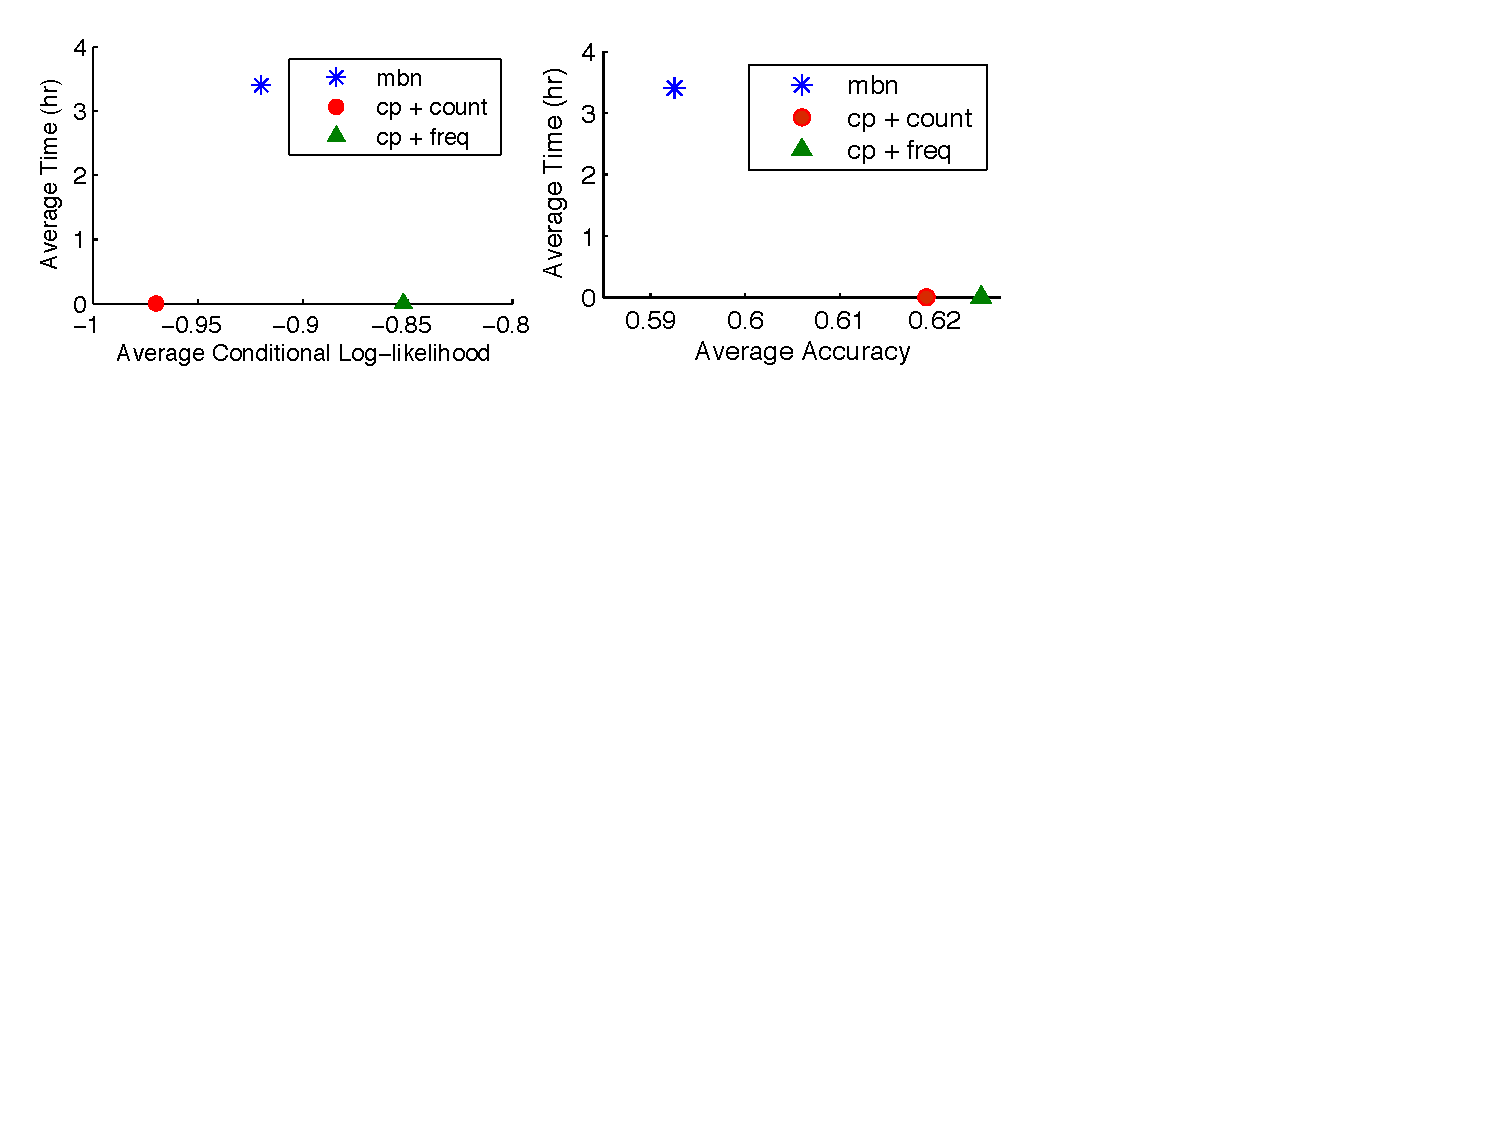
\includegraphics[width=0.5\textwidth]{summary-avg}
%}
\caption{Overall predictive performance against weight learning time, averaged over all benchmark databases. 
%Compared to the Markov Logic methods, Bayes net parameter learning takes essentially no time. 
\label{fig:summarize}}
\end{center}
\end{figure}

\paragraph{Bayes Net Parameter Learning.}
\subparagraph{CLL.} {\em Using frequencies rather than counts improves the conditional log-likelihood score for the log(cp) weights}, substantially on MovieLens and Hepatitis (by 0.4 resp. 0.13 log-likelihood units). Whereas accuracy is a 0-1 loss function, CLL is continuous, so we expect the balancing of factors to have more impact. The log-diff method too improves over the log(cp)+count model on all data sets, though not as much as frequency scaling. These findings support the importance of balancing predictor scales, either through rescaling (frequency) or adjusting weights (log-diff). 

\subparagraph{Accuracy.}  The Bayes net models have quite similar performance; the general ranking trend  [log(cp) + freq] $>$ [log-diff+ count] $>$ [log(cp) + count] holds for this metric as well, with two exceptions: (1) On Hepatitis, the log-diff model has a slightly higher score than the frequency model (about 0.2\%), and (2) on Movielens, the frequency model has a relatively large 3\% advantage. MovieLens is an especially unbalanced set because the number of ratings varies from movie to movie and user to user.  %\marginpar{More details?} 
Also, there are generally many more users rating a given movie than movies rated by a given user. 
%The MBN weights in Figure~\ref{fig:boxplots} also indicate that scale balancing is especially important for MovieLens.

\paragraph{Bayes net vs. Markov net parameters.} 
{\em Bayes net parameters in combination with the frequency/random regression model are competitive with the optimized general weights.} 
 
\subparagraph{CLL.}
The CP+frequency  model scores substantially better than the Markov net weights on Mutagenesis, Hepatitis and MovieLens (by 0.18, 0.11, 0.08 log-likelihood units) but worse on Mondial (0.06 difference). 

%\begin{figure}[htbp]
%\begin{center}
%\resizebox{0.5\textwidth}{!}{
%\includegraphics{summary-cll}
%%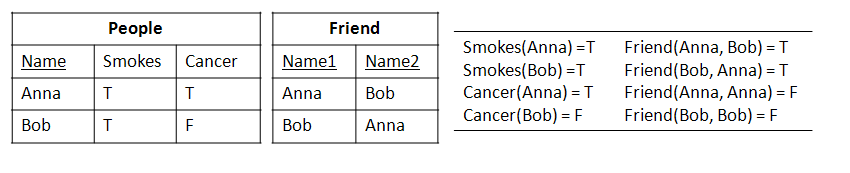
\includegraphics[width=1\textwidth]{database.png}
%}
%\caption{Performance on conditional log-likelihood against time, averaged over all four benchmark databases. \label{fig:summary-cll}}
%\end{center}
%\end{figure}

\subparagraph{Accuracy.} 
The CP+frequency models have a slightly higher score than the Markov net weights, with the biggest differences on MovieLens (5\%) and Hepatitis (4\%). 

%We also performed experiments using the Markov net weights together with the frequency model.
%There is little difference between the Markov model with counts and frequencies. We hypothesize that this is because the optimized Markov model weights include a scaling component. 
%This hypothesis is 
%%Figure~\ref{fig:boxplots} examines 
%confirmed by the scaling components of the weights directly; we omit the details due to space constraints. \marginpar{go back to scaling effects}



%The scaling effects are especially strong for MovieLens, where the Bayes net frequency model outperforms the count model the most.
%
%Every dataset shows scaling effects except for UW, where all methods achieve the same CLL score. The scaling effects are especially strong for MovieLens, where the Bayes net frequency model outperforms the count model the most.
%
%
%\begin{figure}[htbp]
%\begin{center}
%%\resizebox{0.5\textwidth}{!}{
%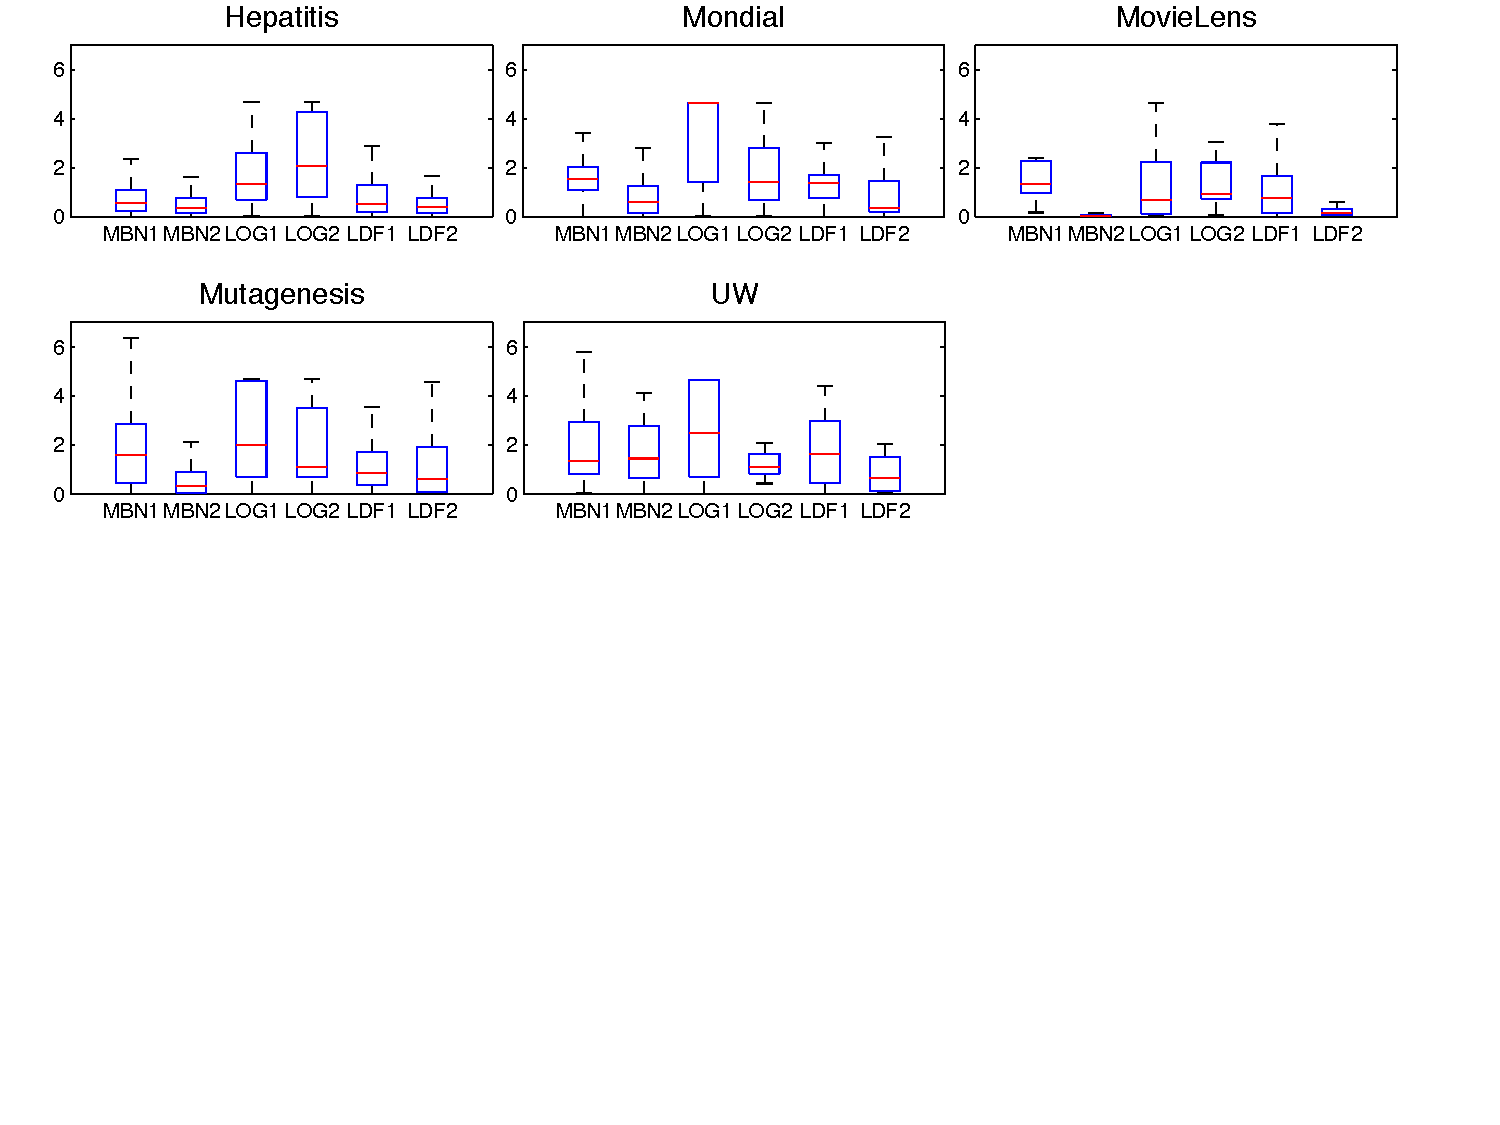
\includegraphics[width=1\textwidth]{boxplots}
%%}
%\caption{Boxplots of the absolute weight sizes learned by the Markov Logic Network method. The median weight size is shown for the set of clauses with one 1st-order variable (left), and the set of clauses with two 1st-order variables (right). Smaller weights for 2-variable clauses balance their larger number of groundings against the smaller number for one-variable clauses.
%\label{fig:boxplots}}
%\end{center}
%\end{figure}


%For the Markov net methods, both count and frequency models have almost the same scores, which is evidence that the learned parameters include scaling components. 
%Overall our experiments provide good evidence that the frequency model using Bayes net conditional probabilities is competitive with a general Markov net log-linear model.


%The next section presents synthetic-data experiments that focus on the scaling effect. 

%\subsubsection{Learning Times.}
%hline Database & Parameters & Complement & FMT & C/FMT \\  \hline \hline
%Mondial & 1618 &157 & 7 &22 \\\hline 
%Hepatitis & 1987 & 18,246 & 77 & 237 \\\hline
%Financial & 10926 & 228,114 & 14,821 &15 \\\hline 
%MovieLens & 326 & 2,070 & 50 & 41 \\ \hline




%\paragraph{Experimental Conclusions.} Compared to Markov Logic parameter learning, Bayes net parameter learning is very fast. The Bayes net parameters were competive with the Markov Logic parameters in terms of predictive performance. Using Bayes net parameters with random/frequency regression outperformed the Markov parameters on all but one dataset on our main metric (CLL). Comparing Bayes net parameters using the frequency vs. count regression, the frequency model has better performance on all datasets on CLL. 
Together with our analysis of the scale balancing problem,
the empirical findings make a good case for recommending the frequency model over the count model when the Bayes net parameters are used to derive log-linear weights.



%\begin{figure}[htbp]
%\begin{center}
%\resizebox{0.5\textwidth}{!}{
%\includegraphics{results-summary}
%%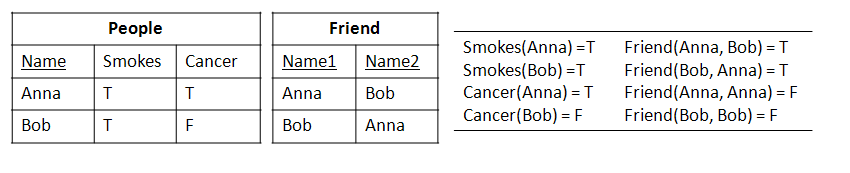
\includegraphics[width=1\textwidth]{database.png}
%}
%\caption{A quick summary of our experimental findings in terms of the average performance over all four benchmark databases. $x$-axis numbers further away from the origin indicate better performance. 
%%The Bayes net parameter methods take next to no time compared to optimizing parameters using Markov Logic procedures. Their predictive performance is better on average than that of the optimized parameters, with the frequency model outperforming the count model.
%\label{fig:summarize}}
%\end{center}
%\end{figure}


%One of the reasons for the widespread popularity of Bayes nets for nonrelational data is that parameters have a natural interpretation and high-quality estimates can be obtained quickly. 
%We believe that providing users with a relational model class that has similar advantages will encourage applications of statistical-relational learning. Users have the option to carry out an initial data exploration and deploy more complex methods if the results are promising.


%\subsection{Synthetic Dataset}
%Scaling factors not so unbalanced. Averages over several predicates. Also has to do with attributes included in Markov blanket. Conduct experiment with synthetic data for the running example.

\section{Conclusion and Future Work} This paper considered an inference model for Bayes nets applied to relational data, that is well defined in the presence of cyclic dependencies. The key idea is to consider the expected log-linear regression value from a {\em random} instantiation of a node's Markov blanket. We provided an equivalent closed form definition that is a log-linear model, whose predictor variables are scaled to be frequencies in the range [0,1]. We compared random regression with standard log-linear models, using as weights both empirical conditional probabilities and weights learned by local optimization. 
The log-conditional probabilities are much faster to compute, typically seconds vs. hours. The predictive performance of log-conditional probability weights was competitive with optimized regression weights, in fact superior on all but one dataset. Overall, random regression appears to be a principled, fast, and accurate model for relational prediction with Bayes nets.
%
%PBNs have been extended with decision trees to obtain more compact models of the conditional distribution of a child node given its parents \cite{Khosravi2012}. This is a natural extension for testing the random regression model; we hypothesize that scaling is even more important, because decision tree pruning leads to more variation in clause length. The powerful and effective technique of functional gradient boosting \cite{Khot2011} could be applied to learning tree models that augment a Bayes net; gradient boosting is well-suited to learning potential functions for log-linear models. 
%In sum, random regression offers a tractable and intuitive definition of inference for Bayes nets that is well-defined even in the presence of cyclic dependencies. 

\bibliographystyle{siam}
\bibliography{siam}

\end{document}